\documentclass[9pt, aspectratio=169]{beamer}

\usetheme[progressbar=frametitle]{metropolis}
\definecolor{lightgray}{RGB}{50, 60, 60}
\definecolor{pitchblack}{RGB}{0, 0, 0}
\definecolor{lightbeige}{RGB}{255, 251, 241}
\definecolor{mediumgray}{RGB}{200, 200, 200}

\setbeamercolor{background canvas}{bg=white}
%\setbeamercolor{normal text}{fg=lightbeige}
%\setbeamercolor{frametitle}{bg=lightgray, fg=mediumgray}

%\setbeamertemplate{blocks}[rounded][shadow]

%\setbeamercolor{block title}{fg=white,bg=blue!70}
%\setbeamercolor{block body}{bg=blue!20}

\usepackage[utf8]{inputenc}
\graphicspath{{images/}{images/theme/}}
	
\usepackage{tabularx}	
\setbeamertemplate{caption}[numbered]
\setbeamertemplate{footline}[frame number]
\usepackage{algorithm}
\usepackage{algorithmic}
	
\usepackage{amsmath} % assumes amsmath package installed
\usepackage{amssymb}  % assumes amsmath package installed
\usepackage[mathcal]{euscript}
\usepackage{pifont}% http://ctan.org/pkg/pifont
%\usepackage{hyperref}
\usepackage{multirow}
%\hypersetup{colorlinks=true}
\newcommand{\cmark}{\ding{51}}%
\newcommand{\xmark}{\ding{55}}%

\usepackage{bm}
%\usepackage{natbib} %Apa style for citation
\usepackage{bibentry}
\nobibliography*

\newcommand{\footfullcite}[1]{\footnote{\scriptsize{\bibentry{#1}}}}

%% DONNES UTILES A LA PAGE DE TITRE ET AU PIED DE PAGE...
\title{Learning Scene Geometry for Visual Localization in Challenging Conditions}
%\subtitle{Localisation basée image en conditions difficiles par apprentissage de modalités}
\author{\textbf{Nathan Piasco$^{1,2}$}, Désiré Sidibé$^{1}$, Valérie Gouet-Brunet$^{2}$ et Cédric Demonceaux$^{1}$}
\institute{2019 International Conference on Robotics and Automation} % ON SE SERT DE INSTITUTE POUR METTER LE LIEUX DE LA CONF
\date{20/05/2019}

%\definecolor{IGNVert}{RGB}{148, 192,  22}
%\definecolor{IGNGris}{RGB}{112, 119, 122}
%\definecolor{IGNRouge}{RGB}{255, 100, 100}
\usepackage{ragged2e}
\newcommand{\norm}[1]{\left\lVert#1\right\rVert}
\newcommand{\abs}[1]{\left\lvert#1\right\rvert}

\begin{document}

\begin{frame}[plain,c]
	\titlepage
	\begin{minipage}{0.49\textwidth}
	\centering
		\begin{enumerate}
			\item ImViA-VIBOT, 	ERL CNRS  6000,  Universit\'e  Bourgogne Franche-Comt\'e
			\item LaSTIG MATIS, IGN, ENSG, Universit\'e Paris-Est, 	F-94160 Saint-Mand\'e, France
		\end{enumerate}
	\end{minipage}\hfill
	\begin{minipage}{0.49\textwidth}
	\centering
	\begin{tabular}{c c}
		
\includegraphics[width=0.15\linewidth]{images/logos/ign_logo} & 
			
\includegraphics[width=0.15\linewidth]{images/logos/cnrs} \\
					
\includegraphics[width=0.27\linewidth]{images/logos/ubfc} &
							
\includegraphics[width=0.25\linewidth]{images/logos/imvia} \\
	\end{tabular}
	\end{minipage}
\end{frame}

\section{Introduction}

\label{sec:intro}

\begin{frame}{Problem statement}
	\only<1>
	{
	\begin{minipage}{0.75\linewidth}
		\begin{figure}
			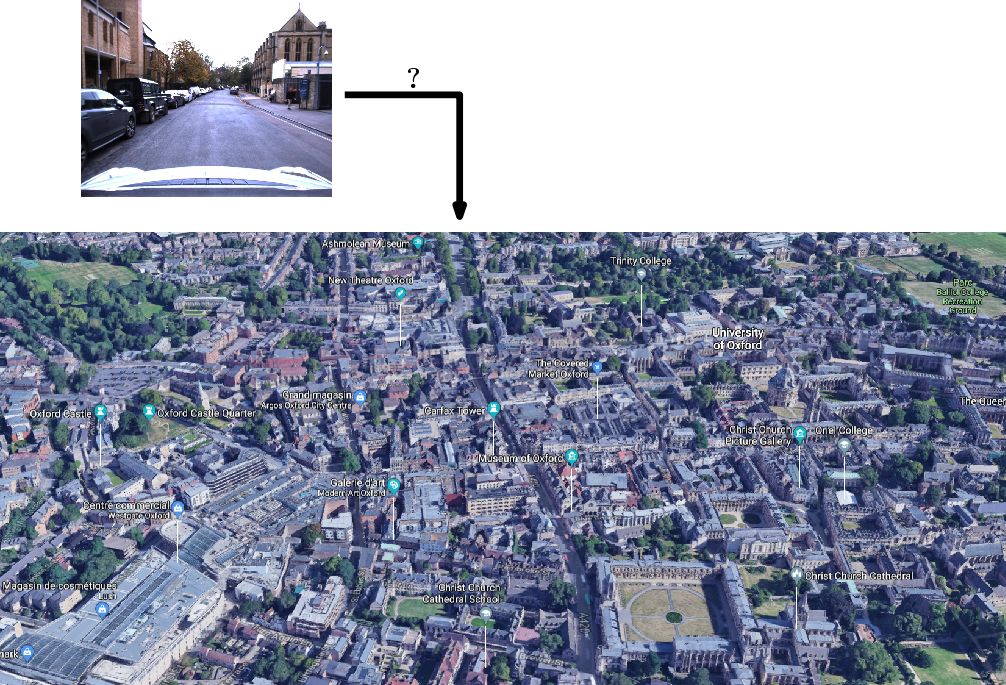
\includegraphics[width=\linewidth]{vect/intro/fig1/gif/1}
		\end{figure}		
	\end{minipage}
	\hfill
	\begin{minipage}{0.18\linewidth}
		We aim to recover the position of an \textbf{unknown query}.	
	\end{minipage}
	}
	\only<2>
	{
	\begin{minipage}{0.75\linewidth}
		\begin{figure}
			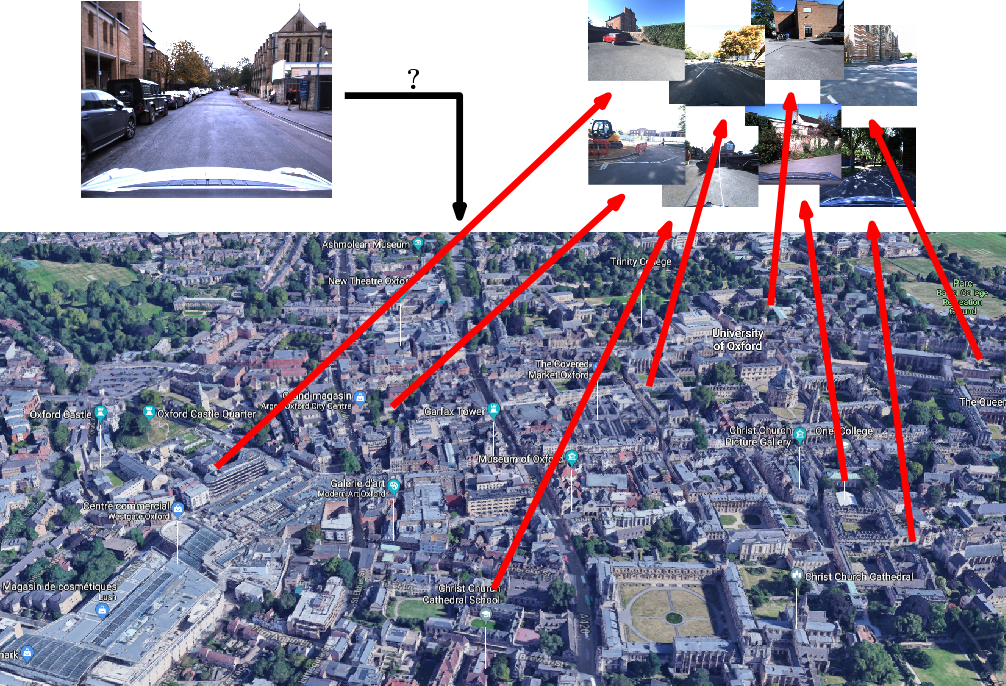
\includegraphics[width=\linewidth]{vect/intro/fig1/gif/2}
		\end{figure}		
	\end{minipage}
	\hfill
	\begin{minipage}{0.18\linewidth}
			We have access to \textbf{geo-localized data}.
	\end{minipage}
	}
	\only<3>
	{
	\begin{minipage}{0.75\linewidth}
		\begin{figure}
			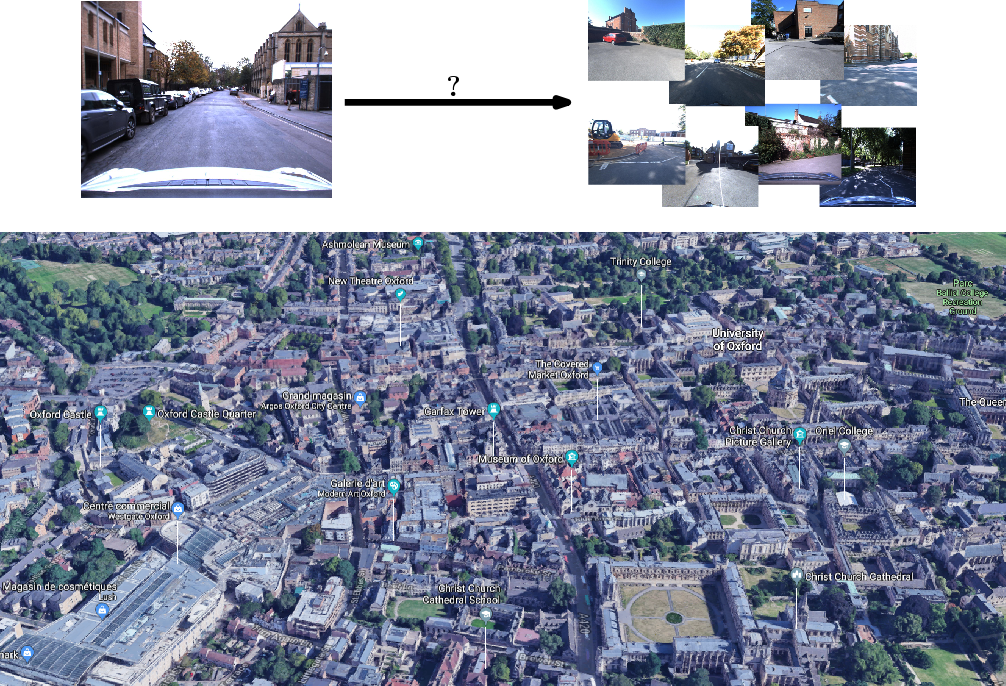
\includegraphics[width=\linewidth]{vect/intro/fig1/gif/3}
		\end{figure}		
	\end{minipage}
	\hfill
	\begin{minipage}{0.18\linewidth}
		We cast the image localisation problem as an \textbf{image-retrieval problem}.
	\end{minipage}
	}
	\only<4>
	{
	\begin{minipage}{0.75\linewidth}
		\begin{figure}
			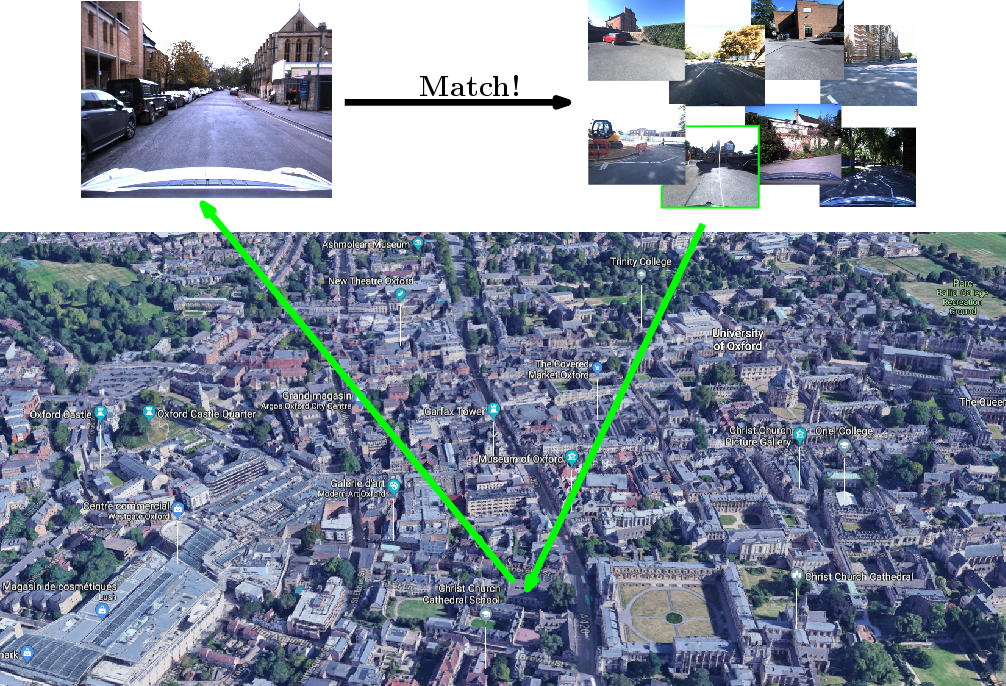
\includegraphics[width=\linewidth]{vect/intro/fig1/gif/6}
		\end{figure}		
	\end{minipage}
	\hfill
	\begin{minipage}{0.18\linewidth}
		We transfer the position of the \textbf{retrieved candidate} to the query.
	\end{minipage}
	}
\end{frame}

\begin{frame}{Challenge in visual based localization}
	\begin{minipage}{0.75\linewidth}
		\begin{figure}
			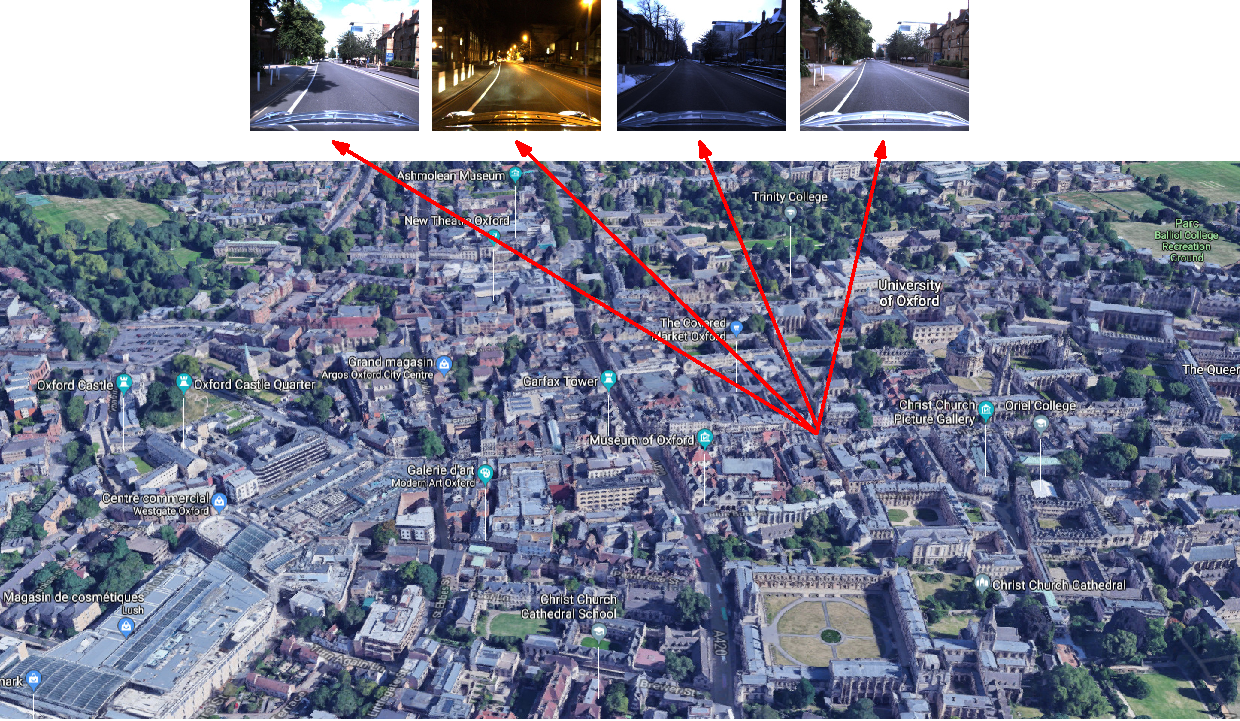
\includegraphics[width=\linewidth]{vect/intro/fig4/1}
		\end{figure}		
	\end{minipage}
	\hfill
	\begin{minipage}{0.18\linewidth}
		Drastic \textbf{visual changes} occur due to season/day-night cycles.
	\end{minipage}
\end{frame}	

\begin{frame}{Geometry to the rescue}
	\only<1>
	{
	\vfill
	\begin{figure}
		\centering
		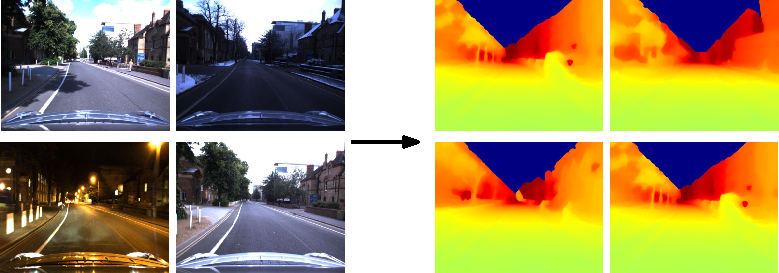
\includegraphics[width=0.8\linewidth]{vect/intro/fig4/2}
	\end{figure}
	\vfill	
	However, \textbf{geometric information} still remains the same.
	}
	\only<2>
	{
	\vfill
	\begin{figure}
		\centering
		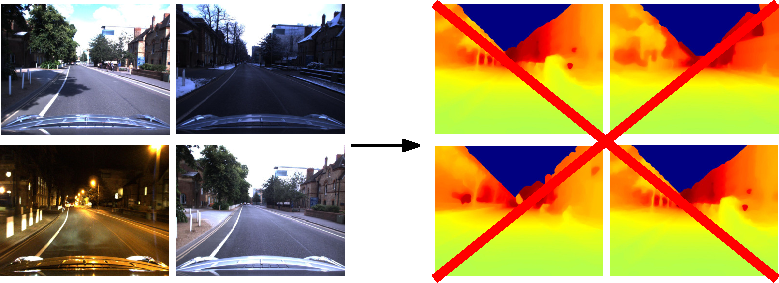
\includegraphics[width=0.8\linewidth]{vect/intro/fig4/3}
	\end{figure}
	\vfill	
	Unfortunately, geometric information is \textbf{not always available}.
	}
	\only<3>
	{
	\vfill
	\centering
	\begin{figure}
		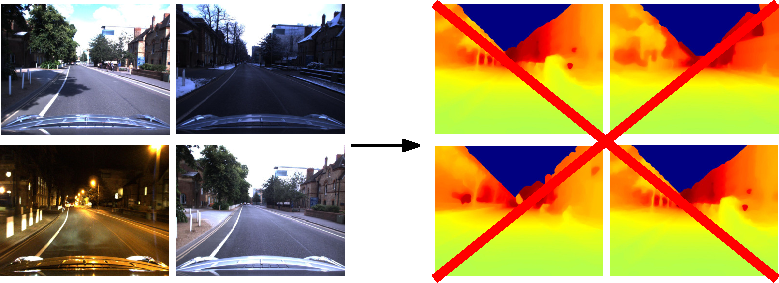
\includegraphics[width=0.6\linewidth]{vect/intro/fig4/3}
	\end{figure}
	\vfill	
	\textbf{How to use partial geometric information to improve image descriptor for localization?}
	}
\end{frame}

\section{{\fontsize{25}{25}\selectfont Learning through missing modality}}

\label{sec:method}
\begin{frame}{CNN as global descriptor}
	\begin{figure}
		
		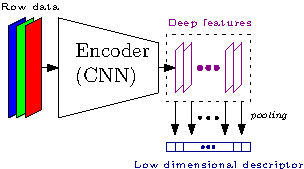
\includegraphics[width=0.5\linewidth]{vect/intro/Desc}
		
		We use a CNN as trainable global image descriptor
	\end{figure}
	\vfill	
	\uncover<2>{CNN global image descriptor can be trained with \textit{triplet loss} function\footfullcite{Arandjelovic2017}.}
\end{frame}


\begin{frame}{Training a descriptor}
	\only<1>
	{
	\begin{figure}
	\centering
	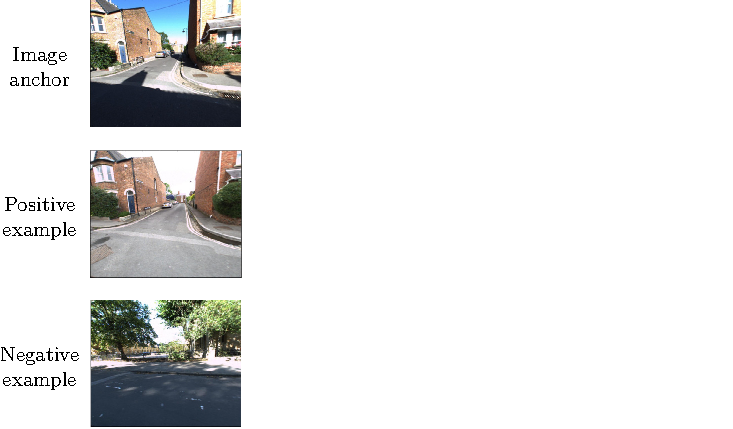
\includegraphics[width=0.7\linewidth]{vect/method/fig2/1}
	\end{figure}
	\vfill
	\textbf{Positive example}: same scene as anchor.
	
	\textbf{Negative example}: unrelated to anchor.
	}
	\only<2>
	{
	\begin{figure}
	\centering
	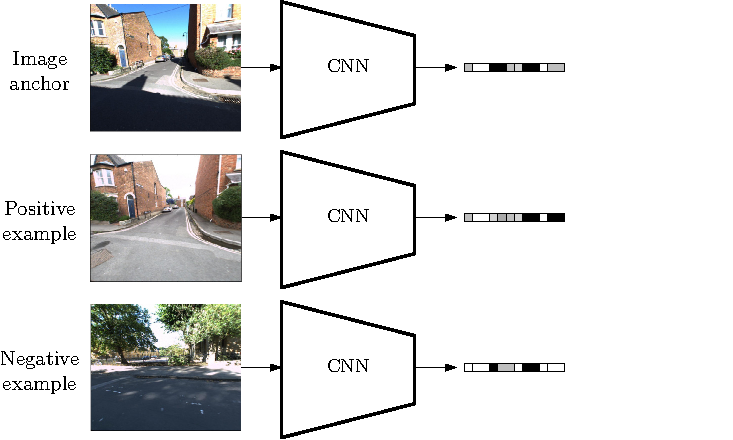
\includegraphics[width=0.7\linewidth]{vect/method/fig2/2}	
	\end{figure}	
	\vfill
	Descriptors computed with the \textbf{same}
	
	deep descriptor.
	}
	\only<3>
	{
	\begin{figure}
	\centering
	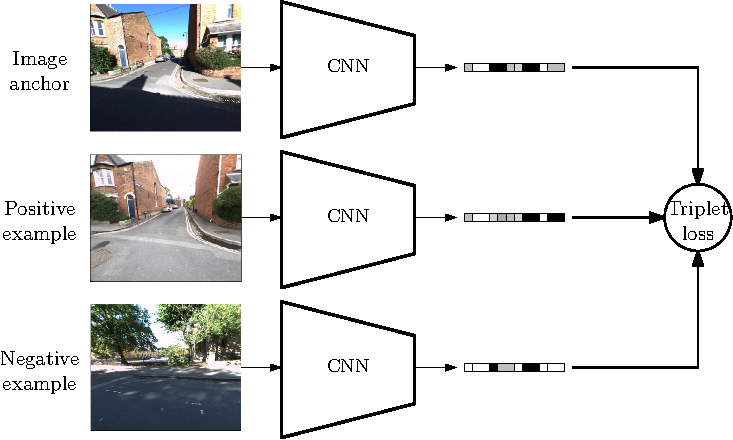
\includegraphics[width=0.7\linewidth]{vect/method/fig2/3}
	\end{figure}	
	\vfill
	\textbf{Triplet loss} penalizes difference between anchor \& positive example and similarity between anchor \& negative example.
	}
%		\uncover<3>{
%			\begin{multline}
%				\label{eq:triplet_loss}
%				Loss_{triplet} = max\left( \norm{f(q) - f(q^+)}^2 - \right. \\
%				\left. \norm{f(q) - f(q^-)}^2 + \lambda, 0\right),
%			\end{multline}
%		}
%		\vfill
%		\only<1>{
%			\begin{align*}
%			with 
%			\begin{cases}
%					f(x) = \textnormal{descriptor of image $x$ } \\
%					q = \textnormal{query image} \\
%			\end{cases}
%			\end{align*}
%		}
%		\only<2>{
%			\begin{align*}
%			with 
%			\begin{cases}
%					f(x) = \textnormal{descriptor of image $x$ } \\
%					q = \textnormal{query image} \\
%					q^+ = \textnormal{positif example} \\
%			\end{cases}
%			\end{align*}
%		}
%		\only<3>{
%			\begin{align*}
%			with 
%			\begin{cases}
%					f(x) = \textnormal{descriptor of image $x$ } \\
%					q = \textnormal{query image} \\
%					q^+ = \textnormal{positif example} \\
%					q^- = \textnormal{negatif example} \\
%					\lambda = \textnormal{triplet loss margin} \\
%			\end{cases}
%			\end{align*}
%		}
%	\end{minipage}
\end{frame}

\begin{frame}{Our method: learning through missing modality}
	\only<1>
	{
	\begin{minipage}{0.6\linewidth}
		\centering
		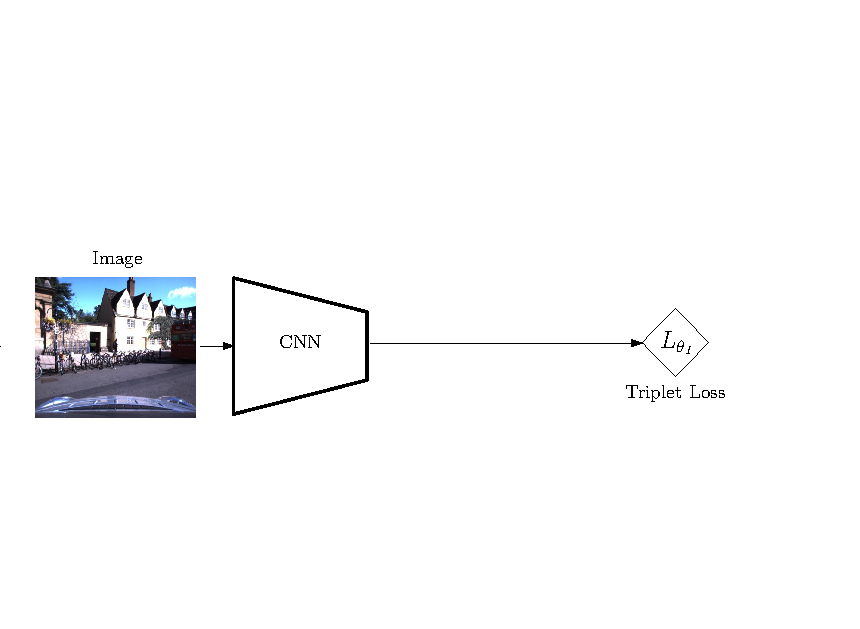
\includegraphics[width=\linewidth]{vect/method/fig3/1}	
	\end{minipage}\hfill
	\begin{minipage}{0.3\linewidth}
		\raggedright
		We use triplet loss to produce strong image descriptor.
	\end{minipage}		
	}
	\only<2>
	{
	\begin{minipage}{0.6\linewidth}
		\centering
		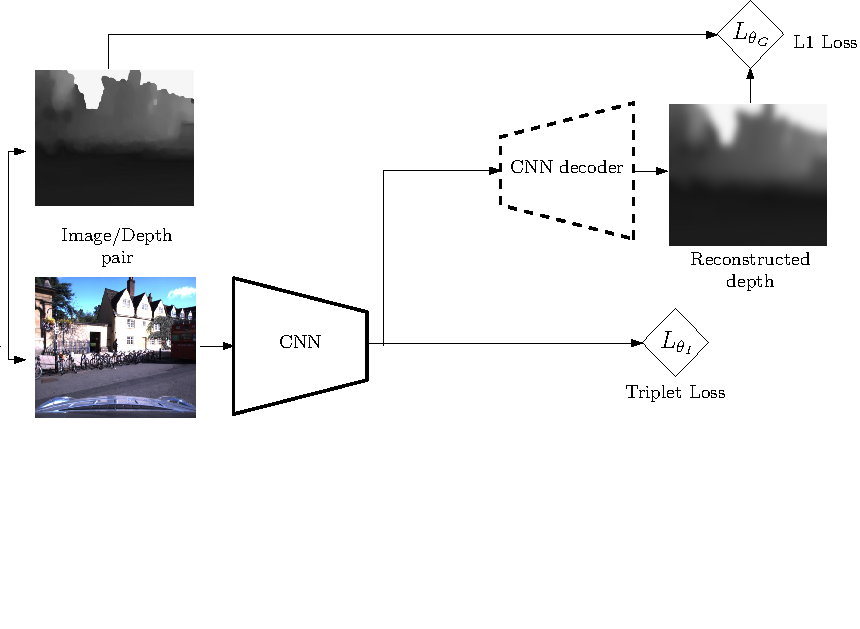
\includegraphics[width=\linewidth]{vect/method/fig3/2}	
	\end{minipage}\hfill
	\begin{minipage}{0.3\linewidth}
		\raggedright
		Latent image representation is given to a CNN decoder to reproduce the scene geometry.\\
		\vspace{0.5cm}
		
		The CNN decoder is simply trained by minimizing $L_{1}$ distance between ground truth and reconstructed depth.
	\end{minipage}		
	
	}
	\only<3>
	{
	\begin{minipage}{0.6\linewidth}
		\centering
		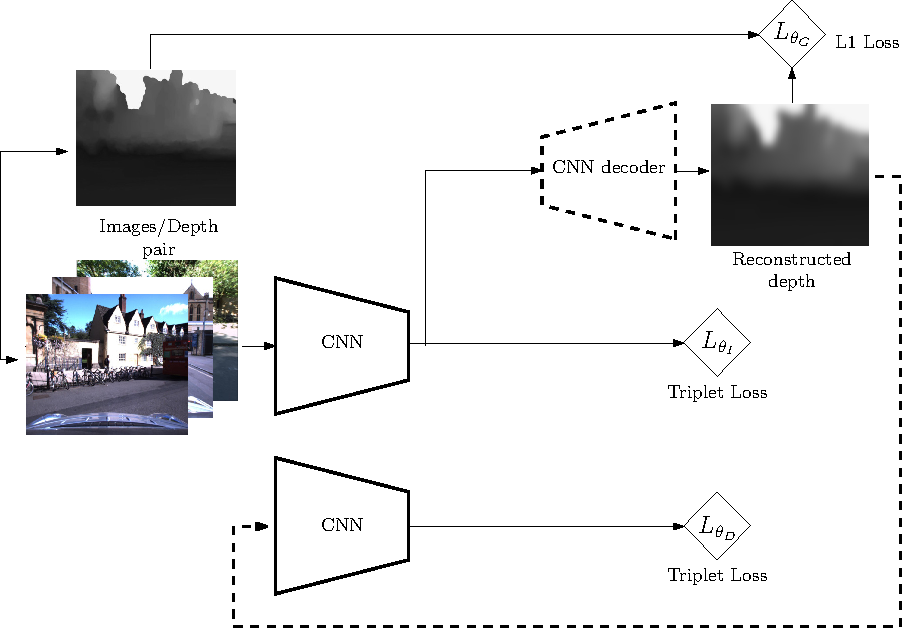
\includegraphics[width=\linewidth]{vect/method/fig3/3}	
	\end{minipage}\hfill
	\begin{minipage}{0.3\linewidth}
		\raggedright
		We use another CNN to produce strong depth map descriptor.
	\end{minipage}			
	
	}
	\only<4>
	{
	\begin{minipage}{0.6\linewidth}
		\centering
		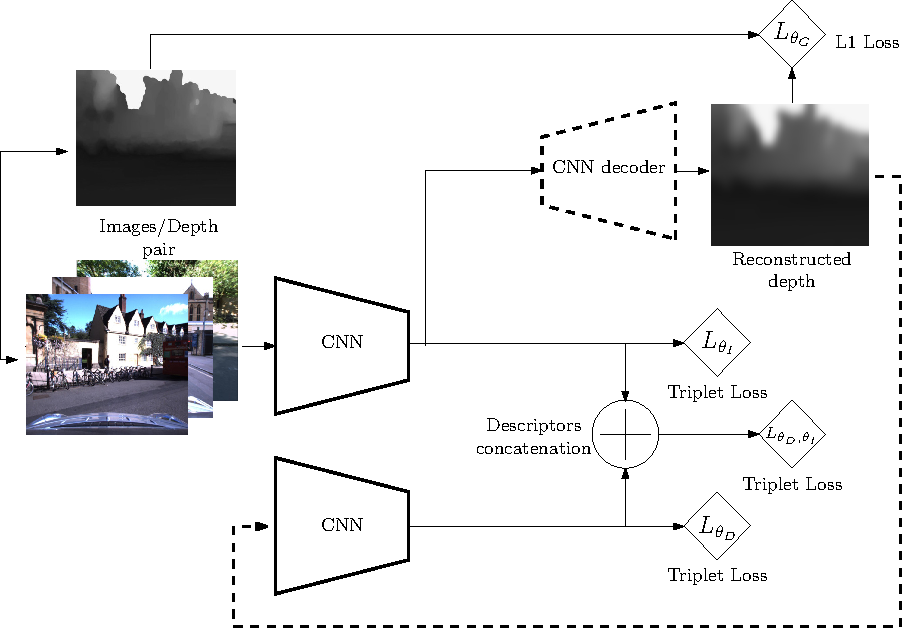
\includegraphics[width=\linewidth]{vect/method/fig3/4}	
	\end{minipage}\hfill
	\begin{minipage}{0.3\linewidth}
		\raggedright
		Final descriptor is obtained by concatenating image and depth map descriptors.
	\end{minipage}			
	
	}
\end{frame}

\begin{frame}{Training policy}
	\only<1>
	{
	\begin{minipage}{0.6\linewidth}
		\centering
		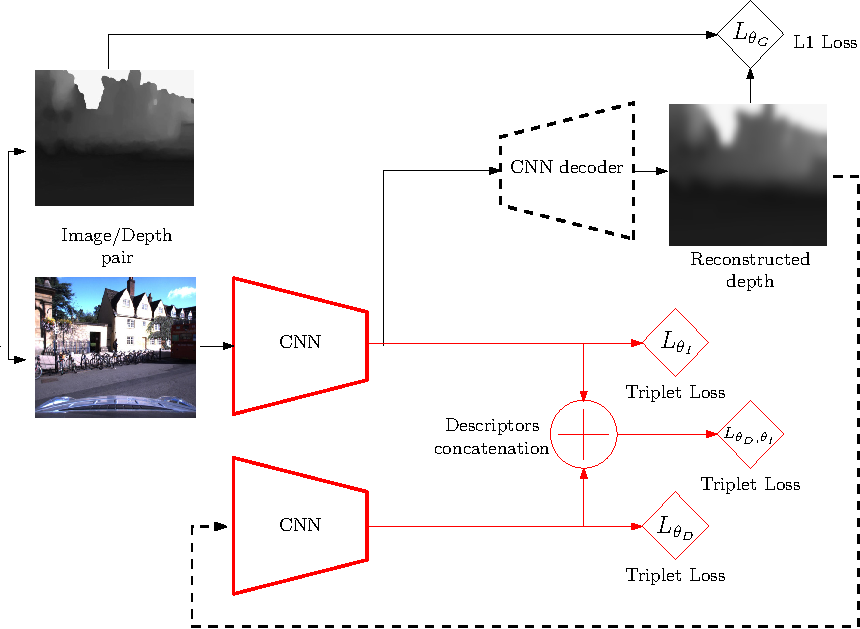
\includegraphics[width=\linewidth]{vect/method/fig3/5}	
	\end{minipage}\hfill
	\begin{minipage}{0.3\linewidth}
		\raggedright
		Data required to train the descriptor part of our system:
		\vspace{0.5cm}
		
		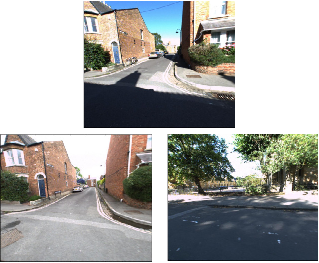
\includegraphics[width=\linewidth]{vect/method/fig3/triplet}	
	\end{minipage}		
	}
	\only<2>
	{
	\begin{minipage}{0.6\linewidth}
		\centering
		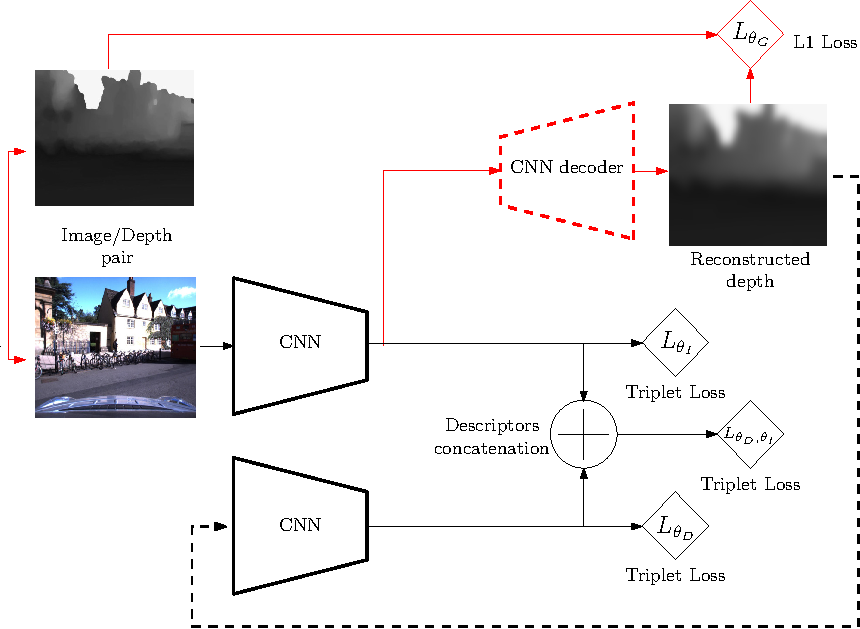
\includegraphics[width=\linewidth]{vect/method/fig3/6}	
	\end{minipage}\hfill
	\begin{minipage}{0.3\linewidth}
		\raggedright
		Data required to train the depth reconstruction part of our system:
		\vspace{0.5cm}
		
		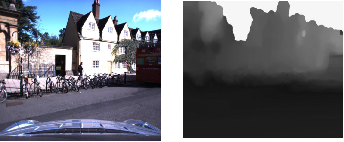
\includegraphics[width=\linewidth]{vect/method/fig3/pair}	
	\end{minipage}			
	}
\end{frame}


\begin{frame}{System deployment}
	\centering
	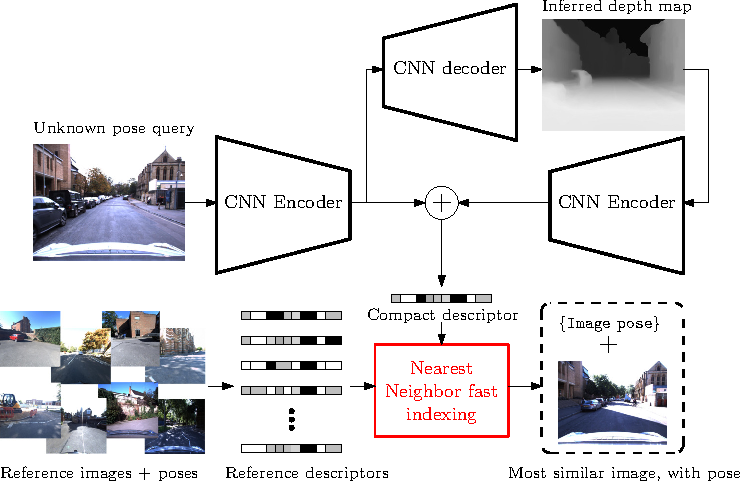
\includegraphics[width=0.7\linewidth]{vect/method/fig4/final}
	\vfill	

	The depth information is only needed during the training step!
\end{frame}
\section{Localization in challenging conditions}

\label{sec:results}

\begin{frame}{Dataset for Localization in challenging conditions}
	
	\begin{minipage}[t]{0.6\linewidth}
		We test our proposal on RobotCar$^1$ dataset with various localization scenarios and different combination of encoders/descriptors.
		\vspace{1cm}
		
		\uncover<3>{
		\textbf{Metric:} we compute the distance between \textbf{the top ranked} returned database image position and the query ground truth position and report the percentage of queries well located under a threshold D.
		}
	\end{minipage}\hfill
	\uncover<2->
	{
	\begin{minipage}[t]{0.32\linewidth}
		\textbf{Competitors:}
		\begin{itemize}
			\item[\textbf{-{}-{}-}] Only RGB [RGB]
			\item[\textbf{-x-}] Hallucination network$^2$ [RGBtD (Hall)]
			\item[\textbf{-o-}] Our proposal [RGBtD (our)]
		\end{itemize}
	\end{minipage}
	\textcolor{white}{\footfullcite{Maddern2016}\footfullcite{Hoffman2016}}	
	}	
\end{frame}

%
%\begin{frame}{Results: cross-season localization}
%	\scriptsize
%	\begin{tabularx}{1.08\linewidth}{X X X X X}
%		Query & NetVLAD (our) & NetVLAD & MAC (our) & MAC \\
%	\end{tabularx}
%	\fboxsep=1pt%padding thickness
%	\fboxrule=1pt
%
%	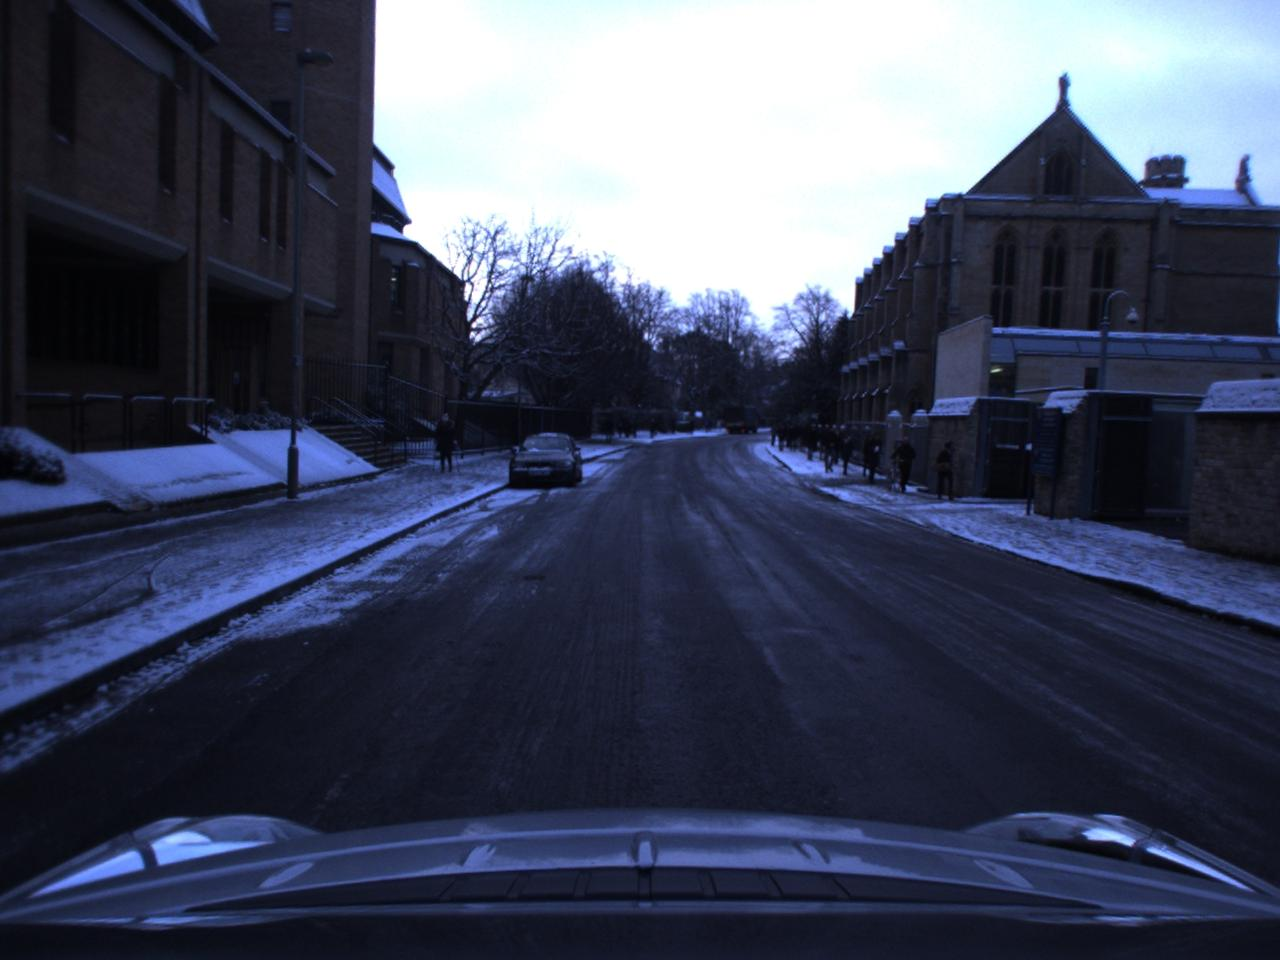
\includegraphics[width=0.12\linewidth]{ims_res/snow/q1/Q.jpg}\hfill
%	\fcolorbox{green}{green}{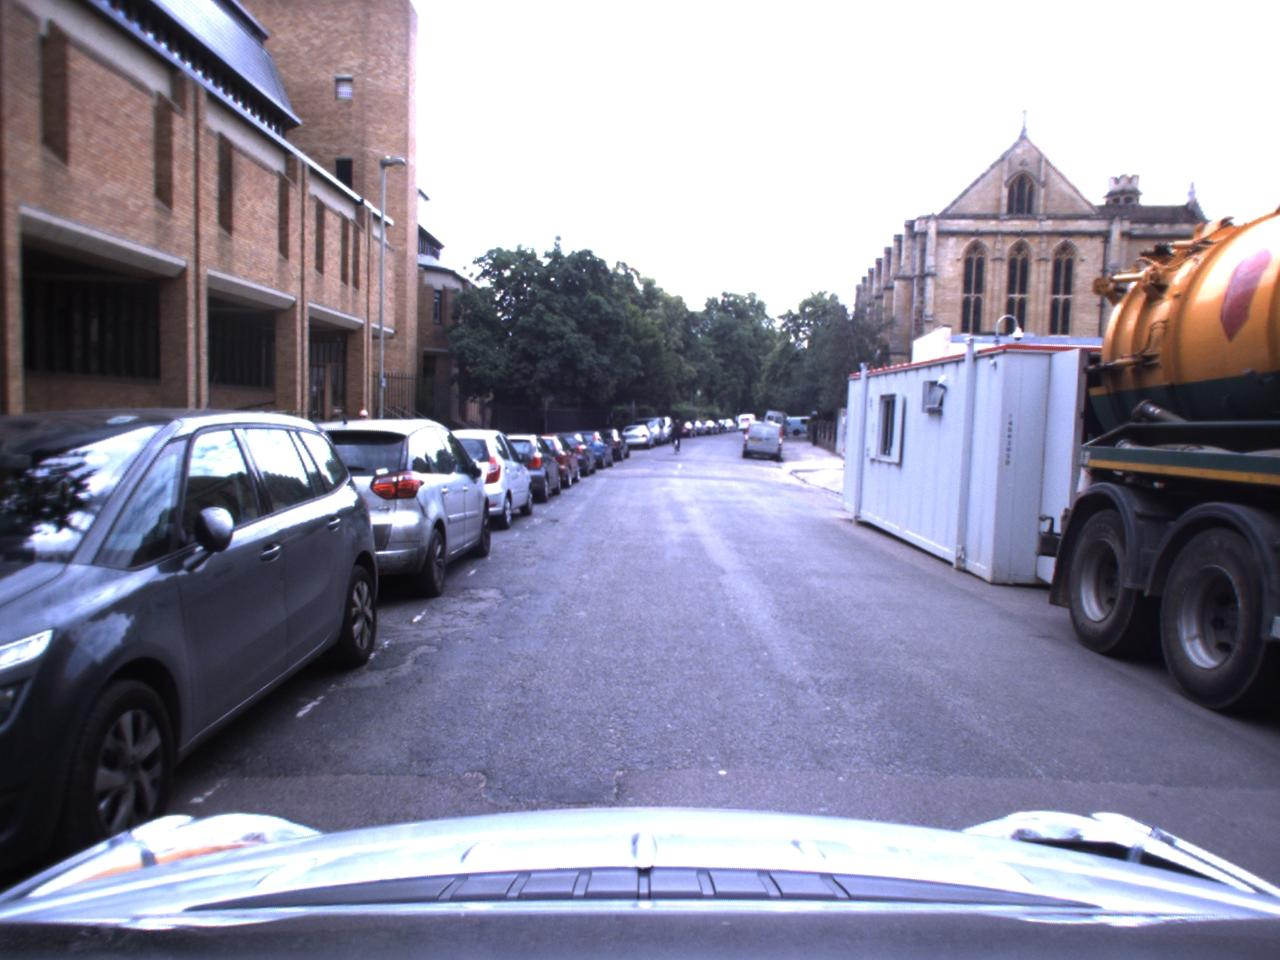
\includegraphics[width=0.12\linewidth]{ims_res/snow/q1/NetVLAD_our.jpg}}\hfill
%	\fcolorbox{red}{red}{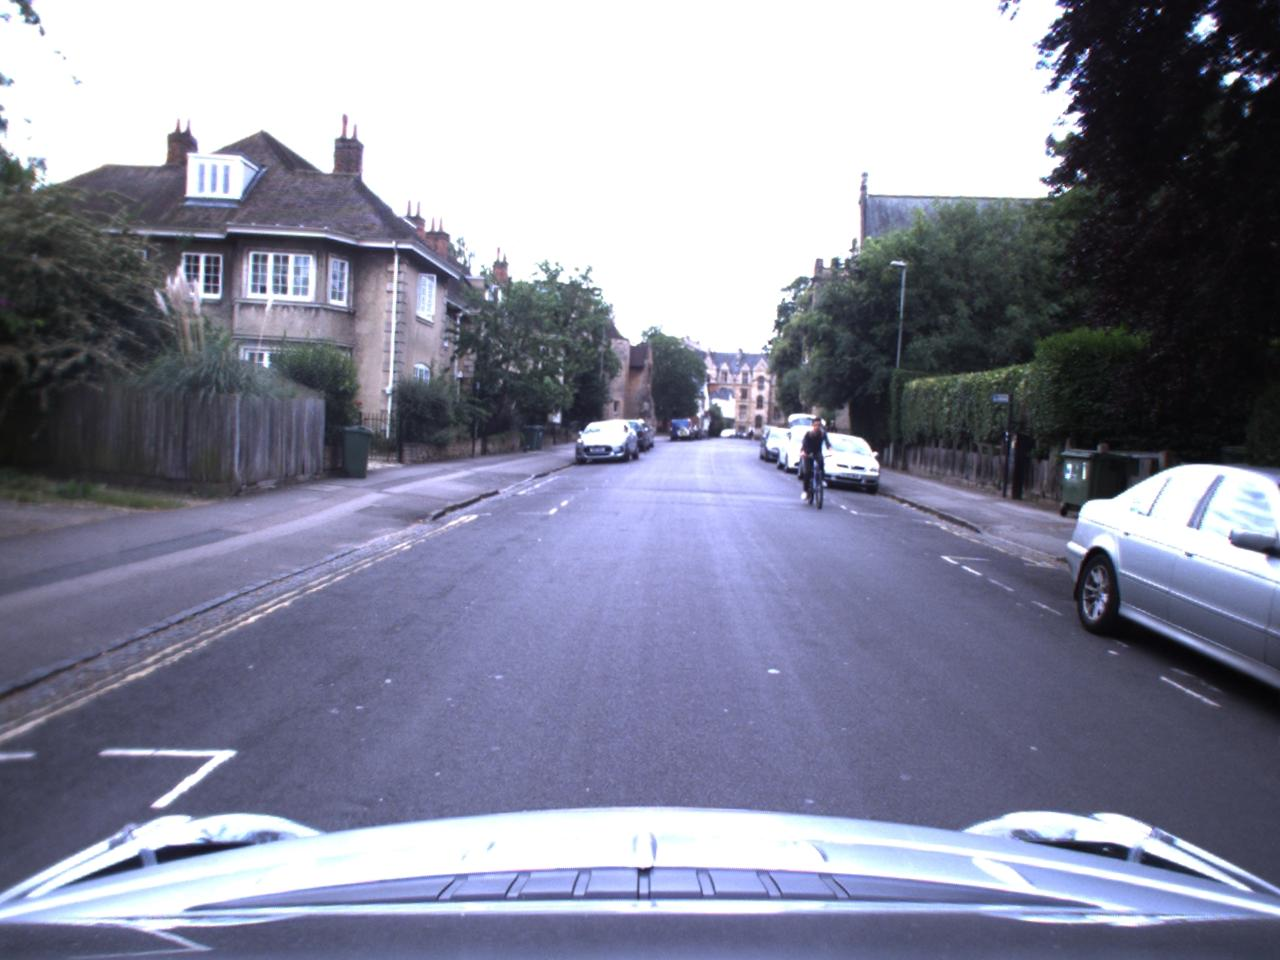
\includegraphics[width=0.12\linewidth]{ims_res/snow/q1/NetVLAD.jpg}}\hfill
%	\fcolorbox{red}{red}{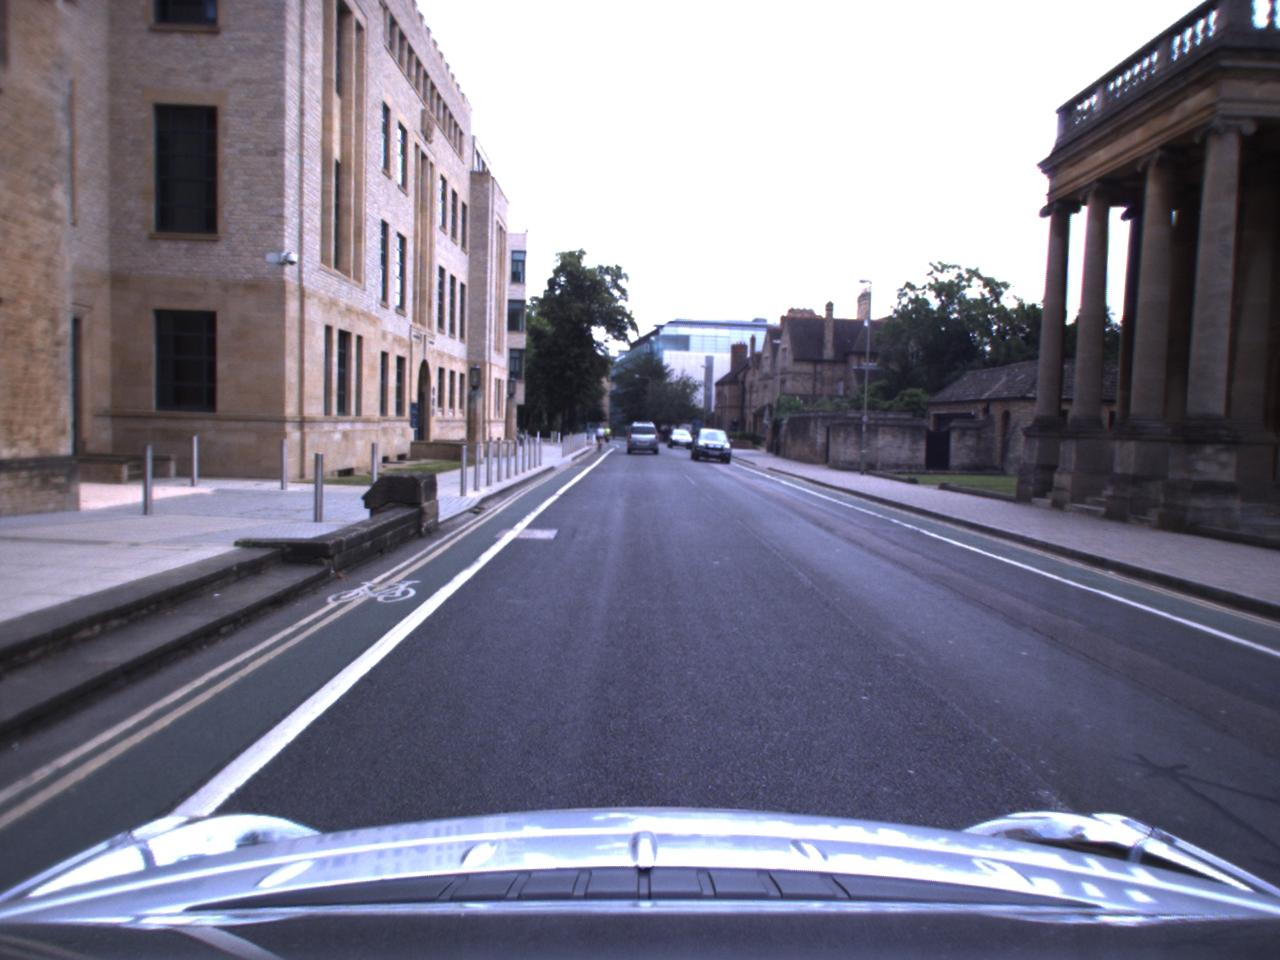
\includegraphics[width=0.12\linewidth]{ims_res/snow/q1/MAC_our.jpg}}\hfill
%	\fcolorbox{red}{red}{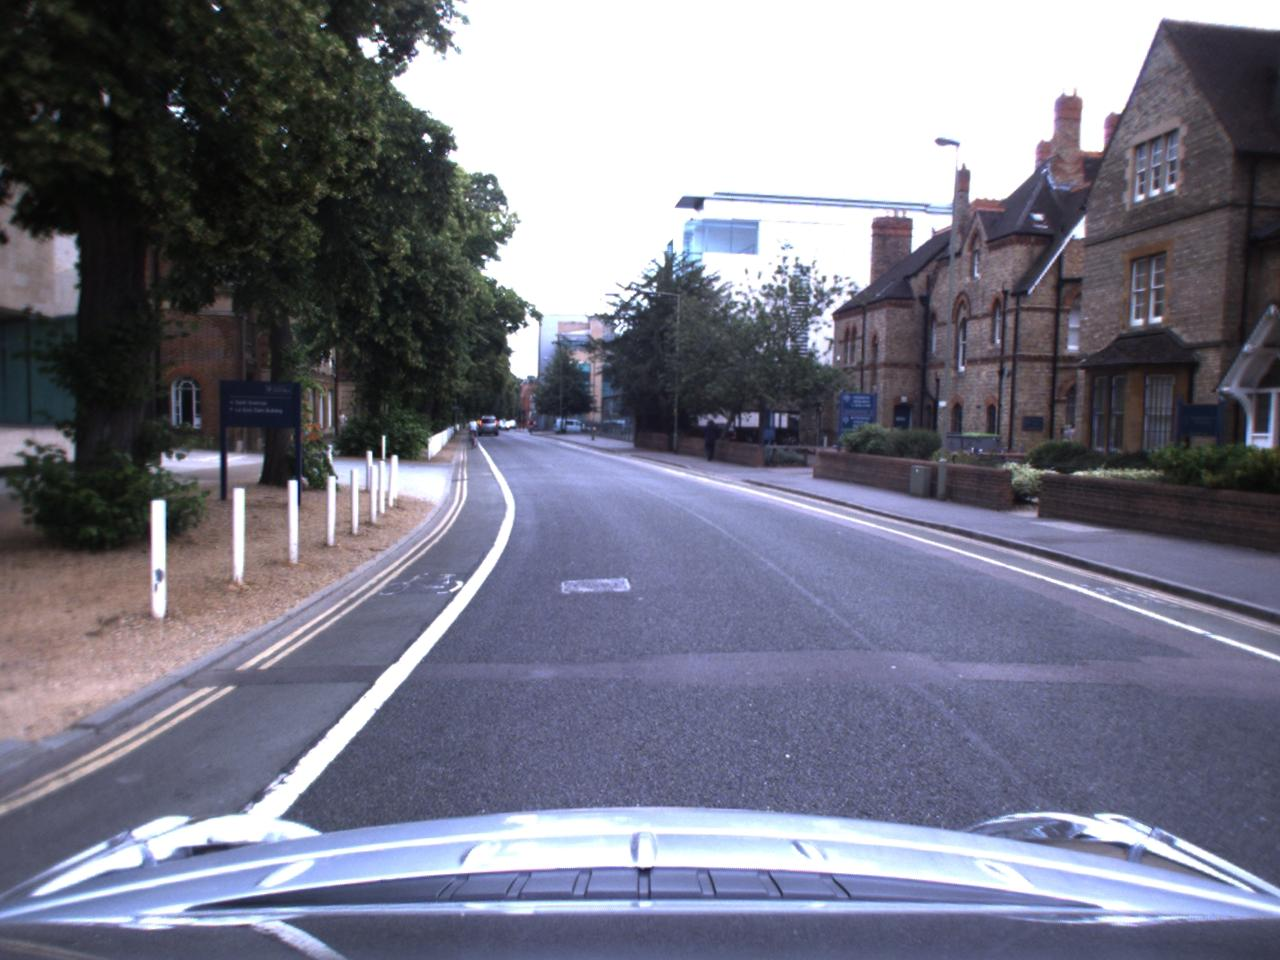
\includegraphics[width=0.12\linewidth]{ims_res/snow/q1/MAC.jpg}}
%	
%	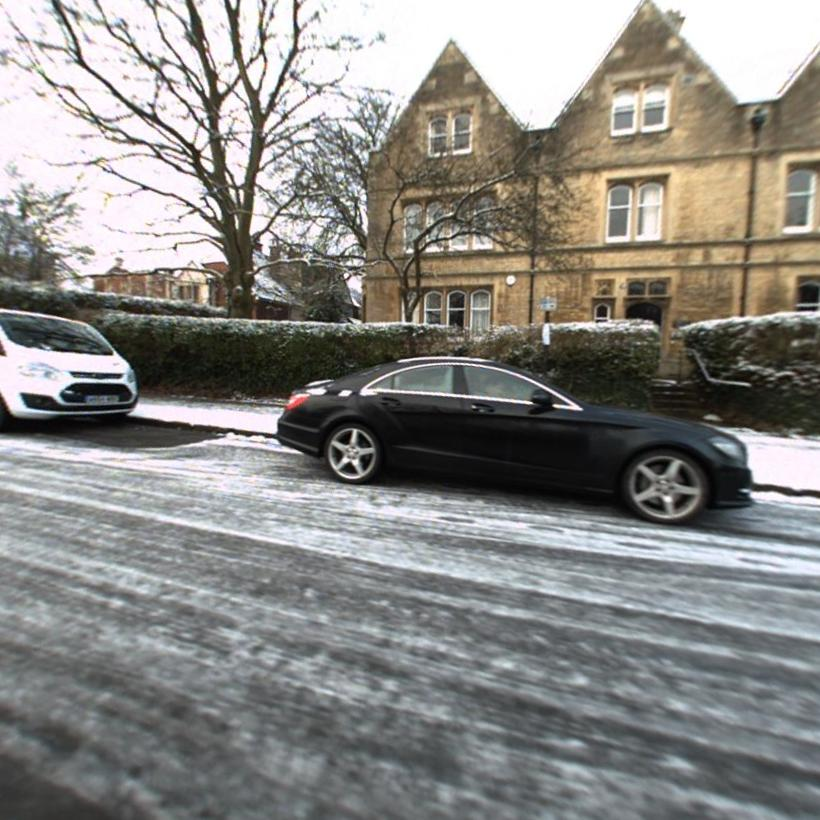
\includegraphics[width=0.12\linewidth]{ims_res/snow/q2/Q.jpg}\hfill
%	\fcolorbox{green}{green}{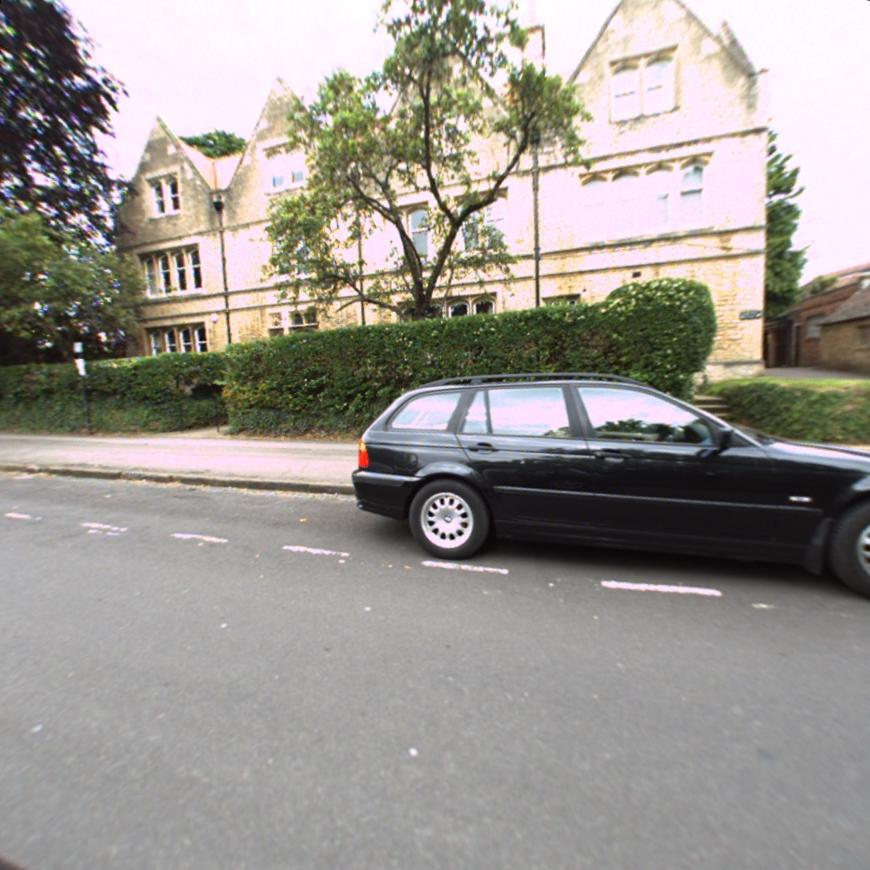
\includegraphics[width=0.12\linewidth]{ims_res/snow/q2/NetVLAD_our.jpg}}\hfill
%	\fcolorbox{red}{red}{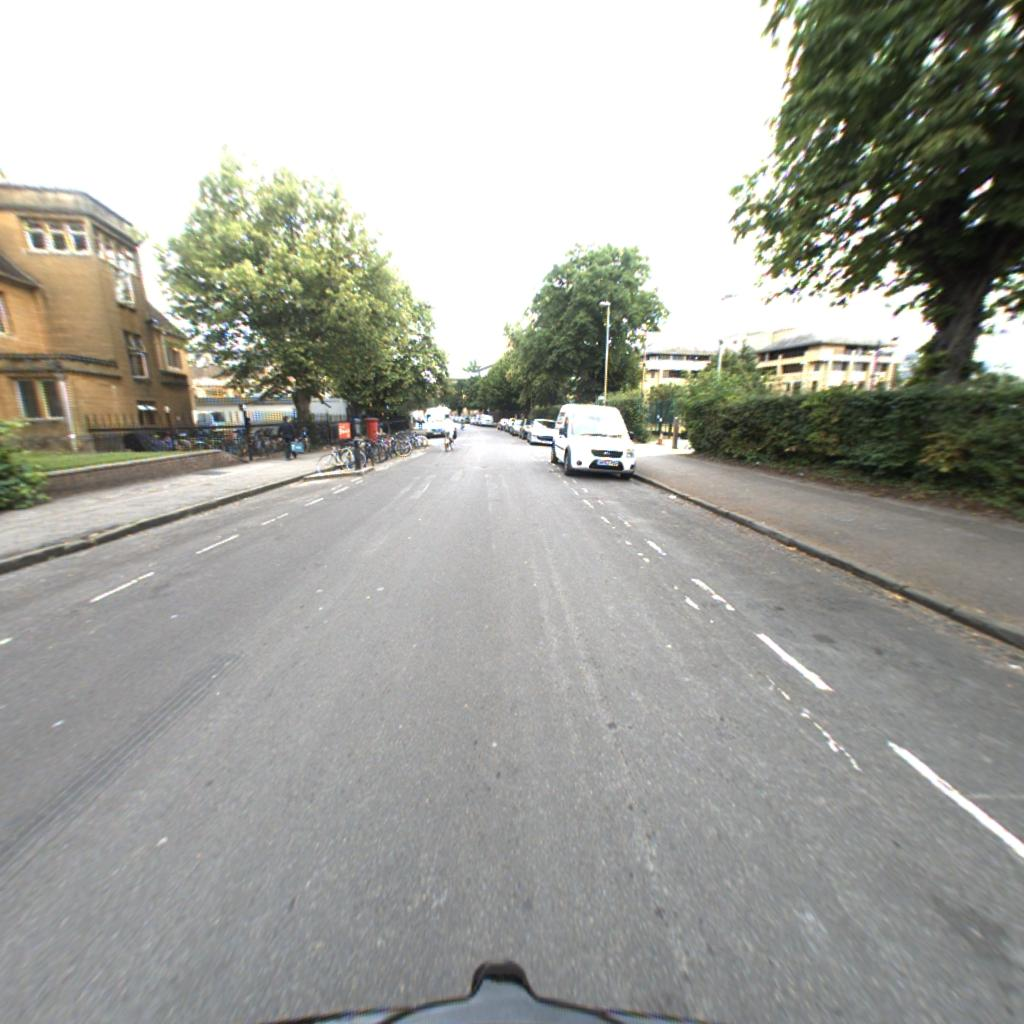
\includegraphics[width=0.12\linewidth]{ims_res/snow/q2/NetVLAD.jpg}}\hfill
%	\fcolorbox{red}{red}{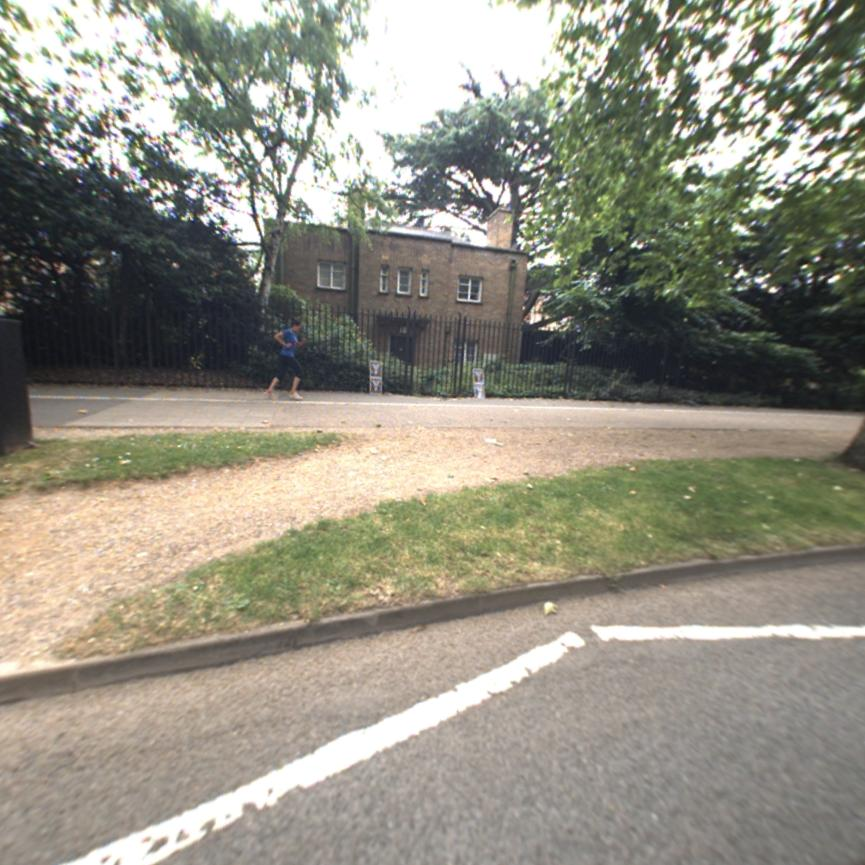
\includegraphics[width=0.12\linewidth]{ims_res/snow/q2/MAC_our.jpg}}\hfill
%	\fcolorbox{red}{red}{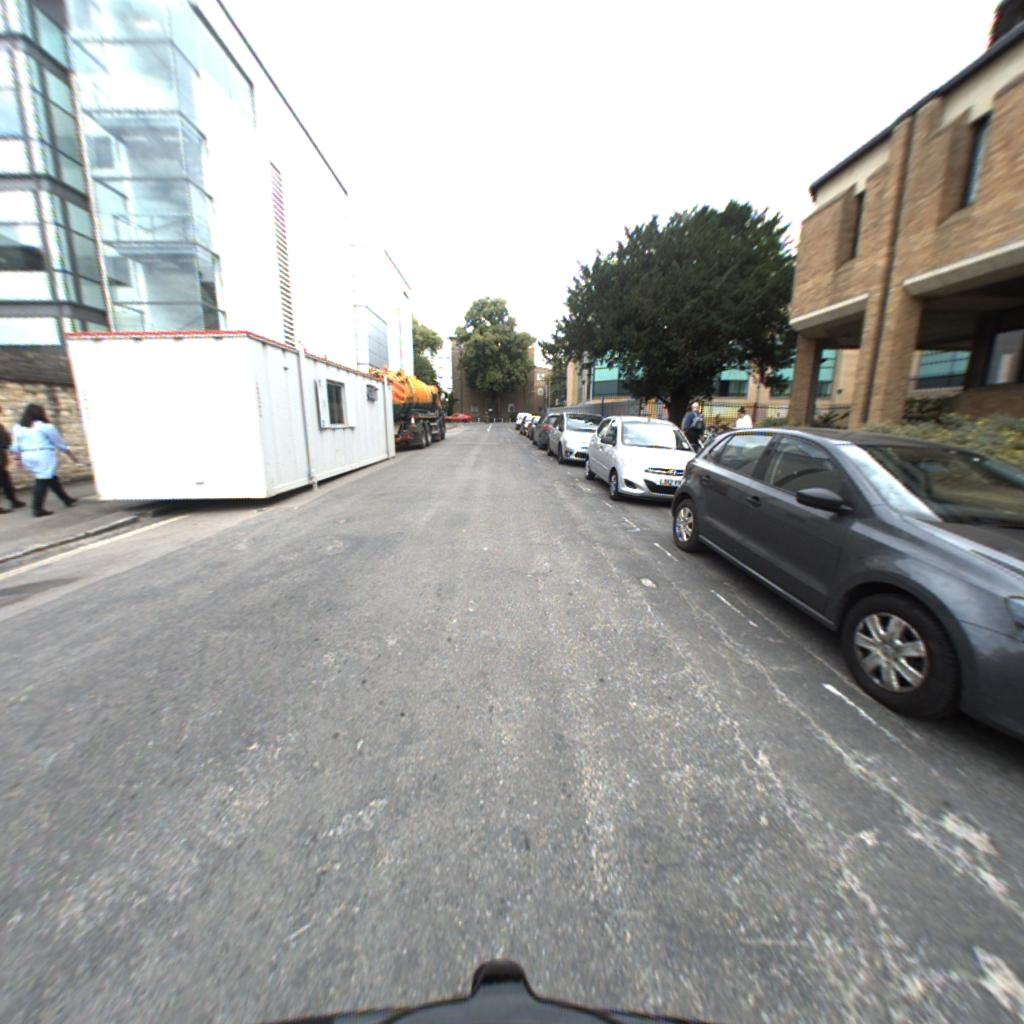
\includegraphics[width=0.12\linewidth]{ims_res/snow/q2/MAC.jpg}}
%	
%	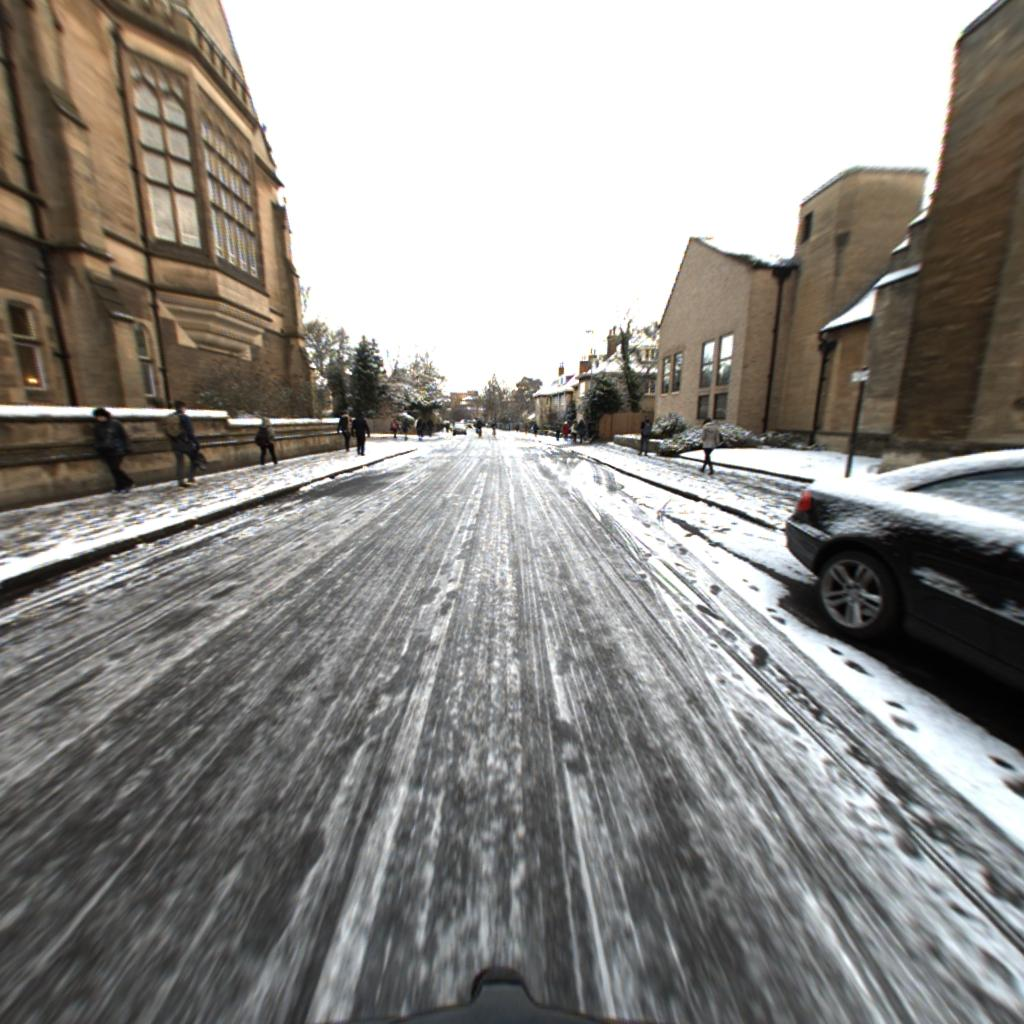
\includegraphics[width=0.12\linewidth]{ims_res/snow/q3/Q.jpg}\hfill
%	\fcolorbox{green}{green}{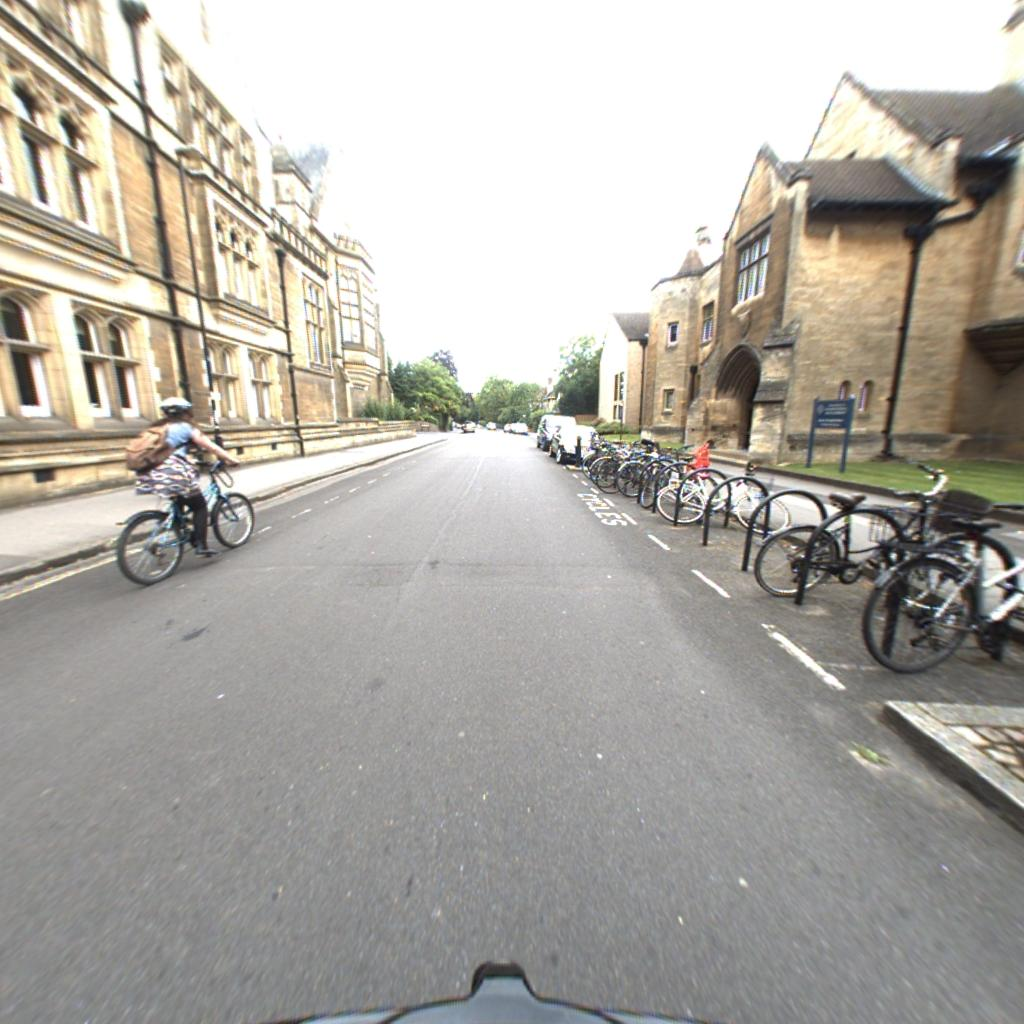
\includegraphics[width=0.12\linewidth]{ims_res/snow/q3/NetVLAD_our.jpg}}\hfill
%	\fcolorbox{red}{red}{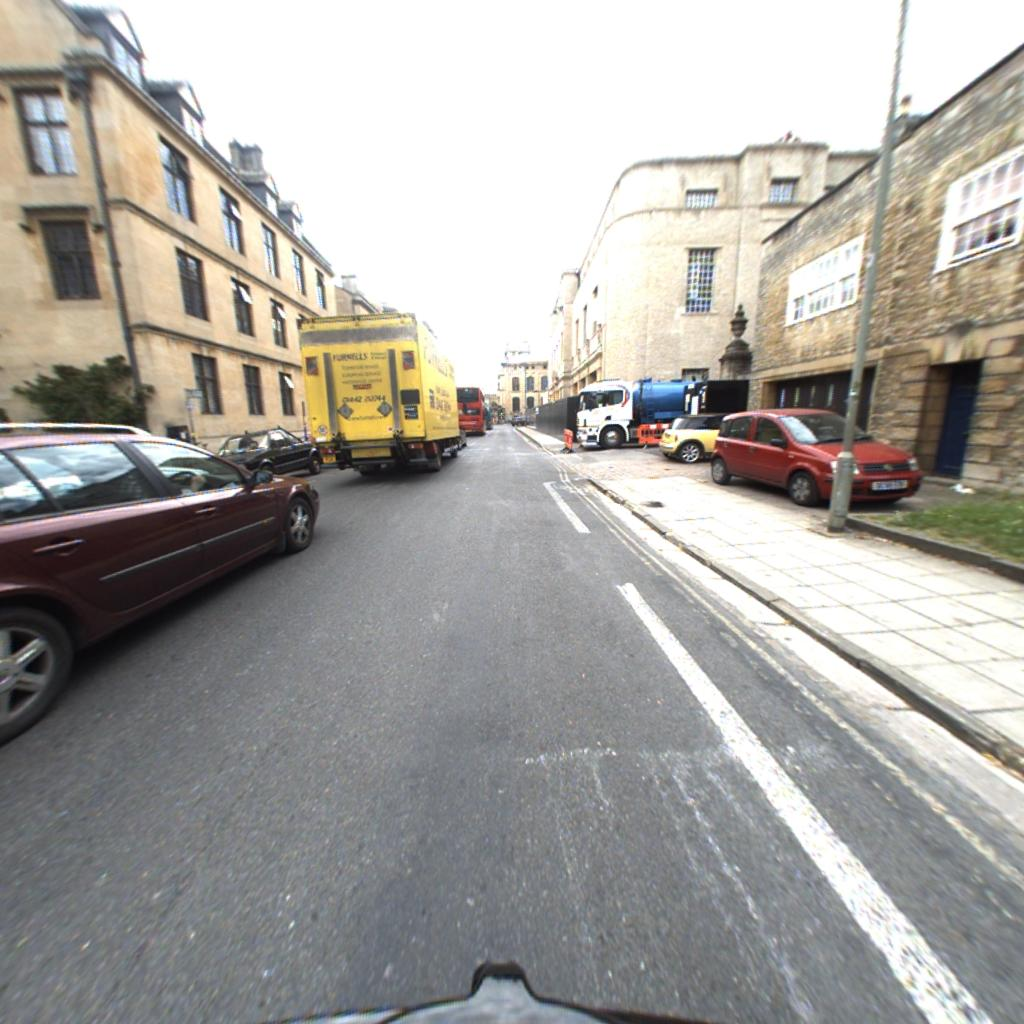
\includegraphics[width=0.12\linewidth]{ims_res/snow/q3/NetVLAD.jpg}}\hfill
%	\fcolorbox{red}{red}{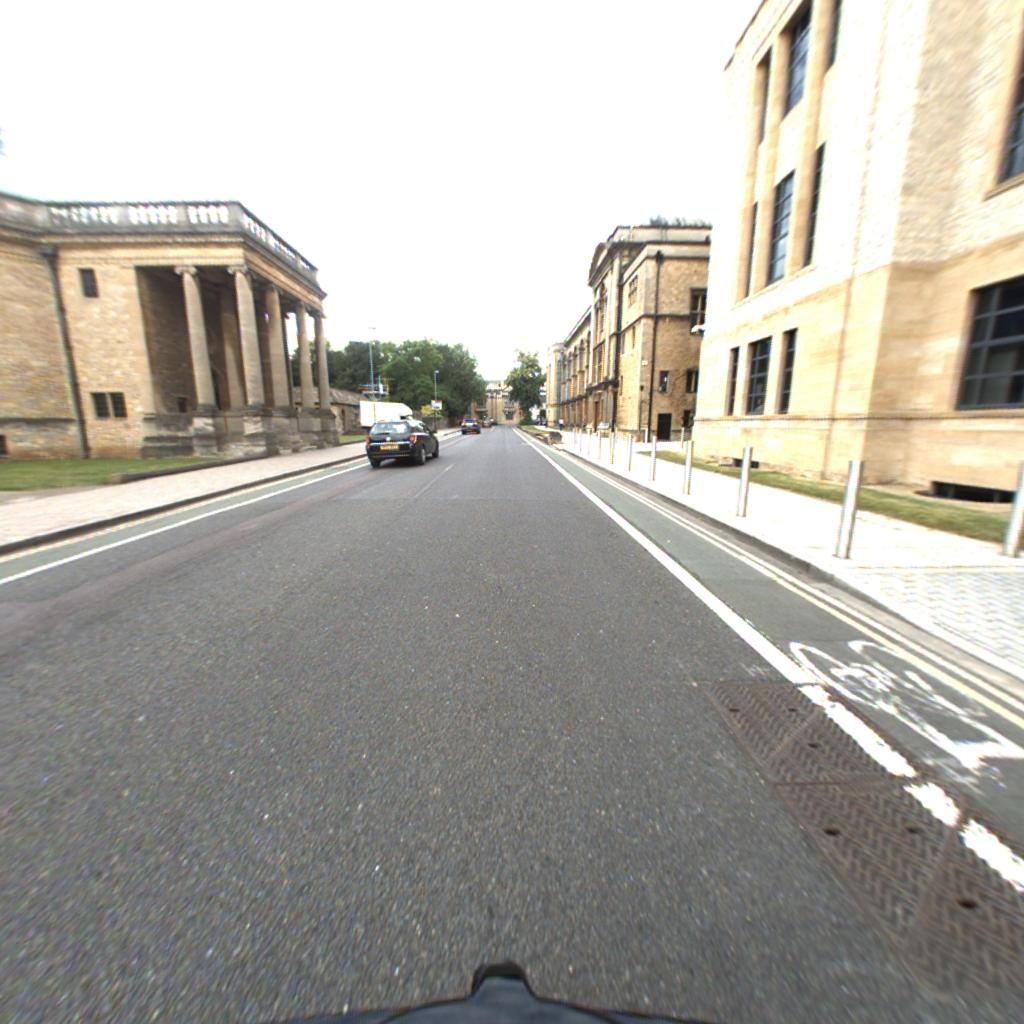
\includegraphics[width=0.12\linewidth]{ims_res/snow/q3/MAC_our.jpg}}\hfill
%	\fcolorbox{red}{red}{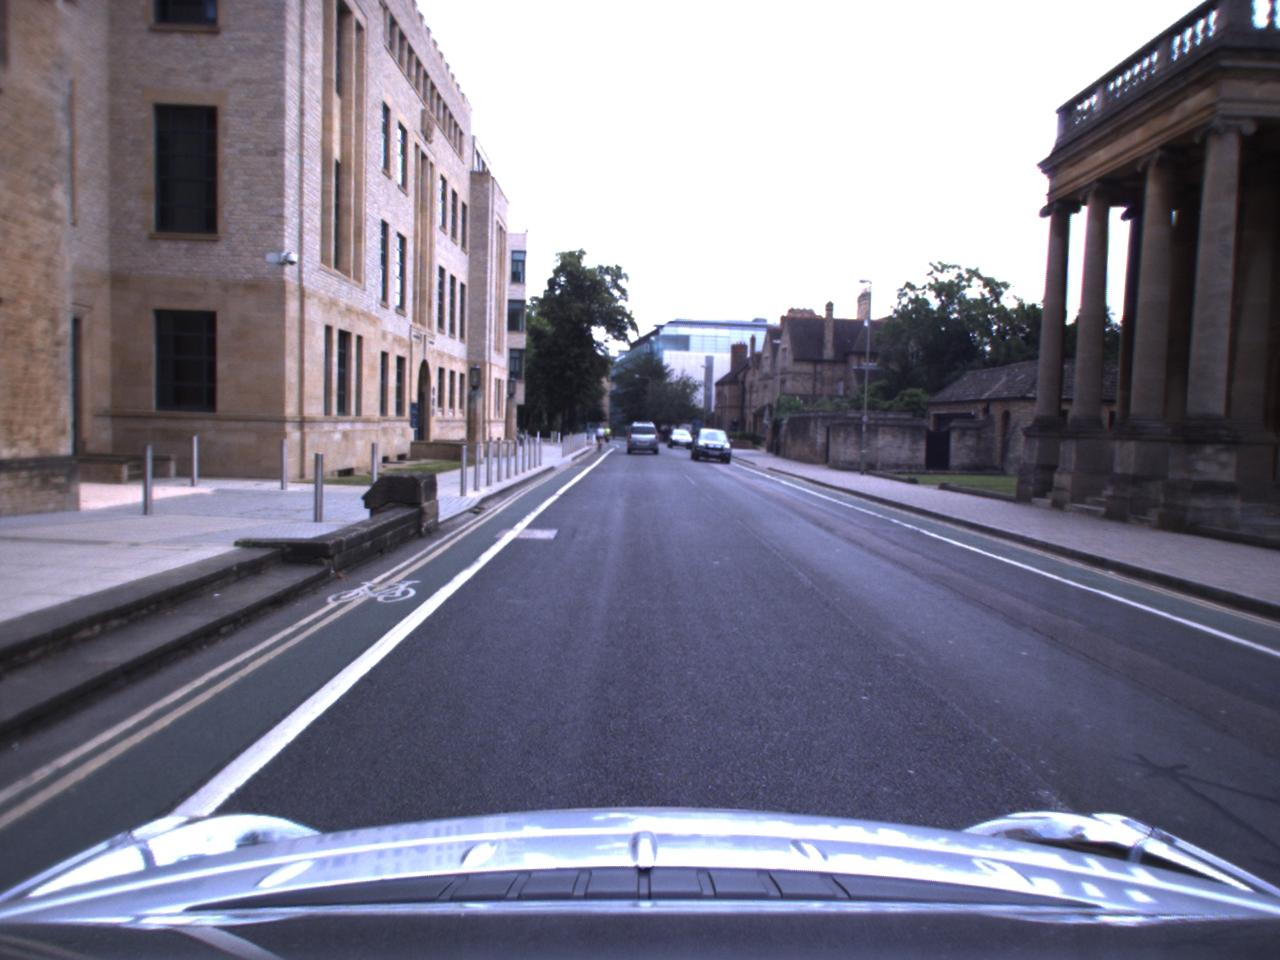
\includegraphics[width=0.12\linewidth]{ims_res/snow/q3/MAC.jpg}}
%	
%	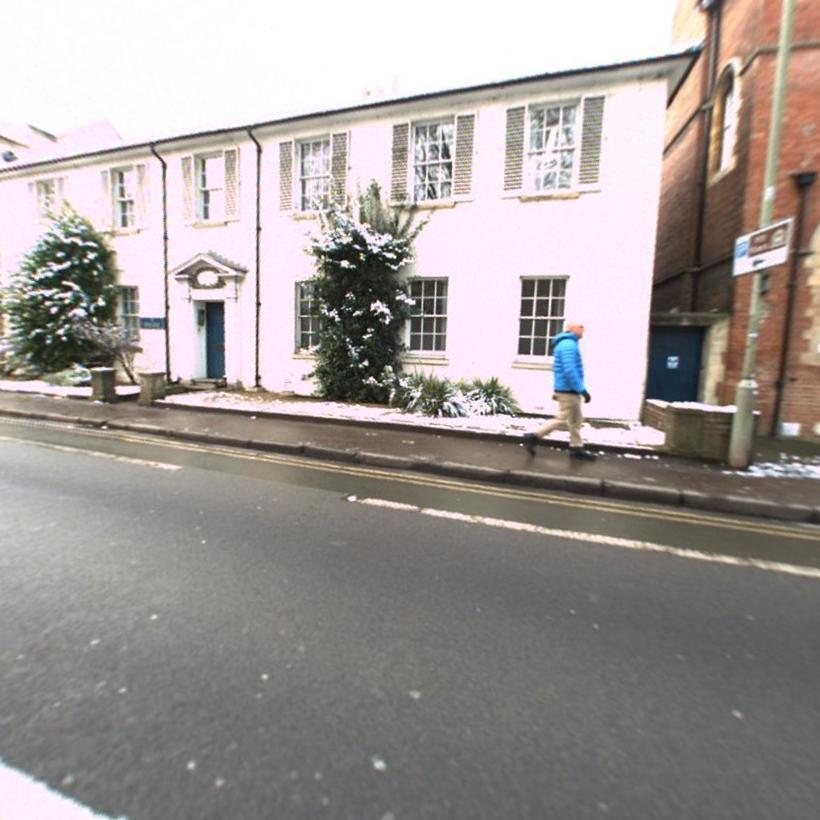
\includegraphics[width=0.12\linewidth]{ims_res/snow/q4/Q.jpg}\hfill
%	\fcolorbox{green}{green}{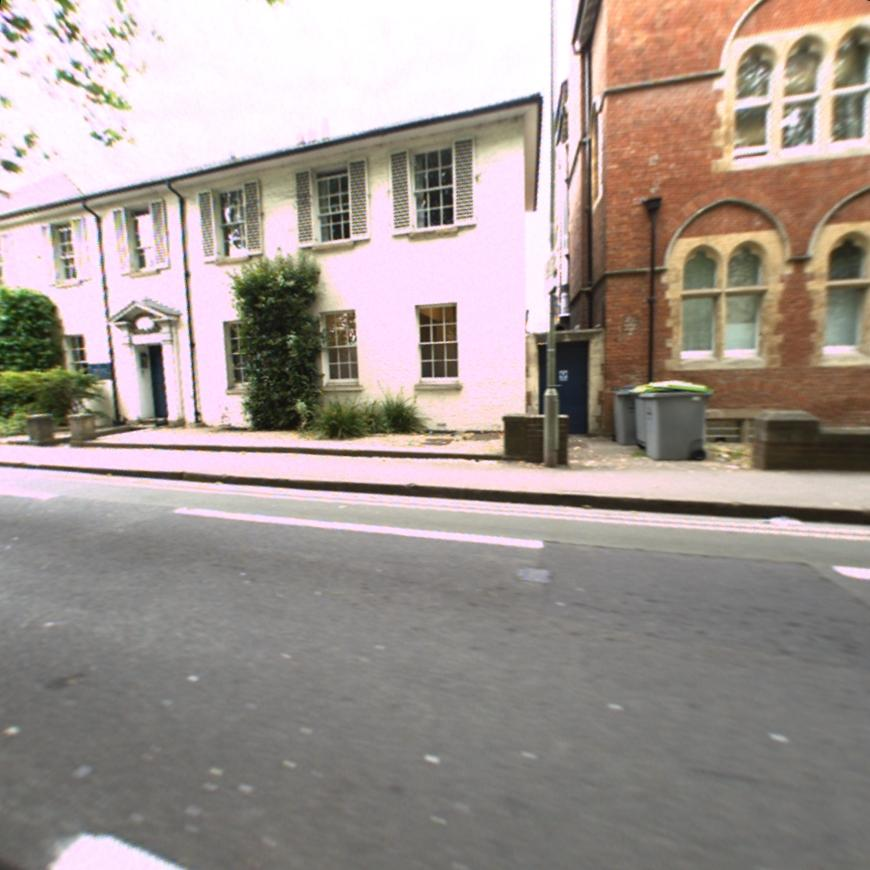
\includegraphics[width=0.12\linewidth]{ims_res/snow/q4/NetVLAD_our.jpg}}\hfill
%	\fcolorbox{green}{green}{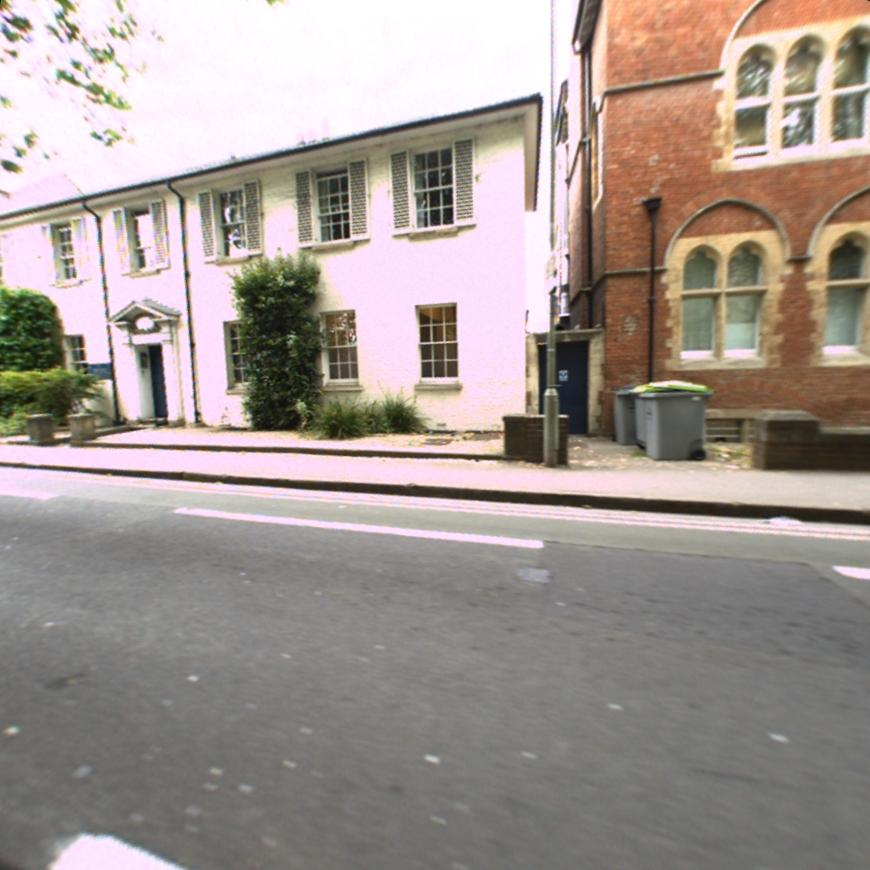
\includegraphics[width=0.12\linewidth]{ims_res/snow/q4/NetVLAD.jpg}}\hfill
%	\fcolorbox{green}{green}{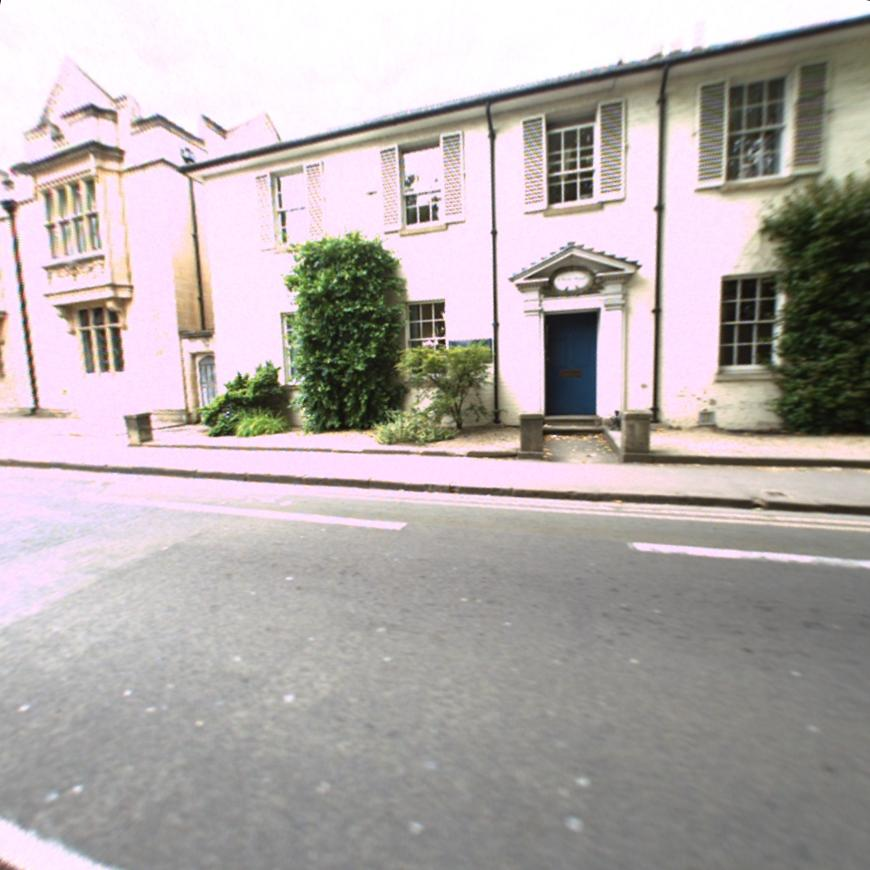
\includegraphics[width=0.12\linewidth]{ims_res/snow/q4/MAC_our.jpg}}\hfill
%	\fcolorbox{red}{red}{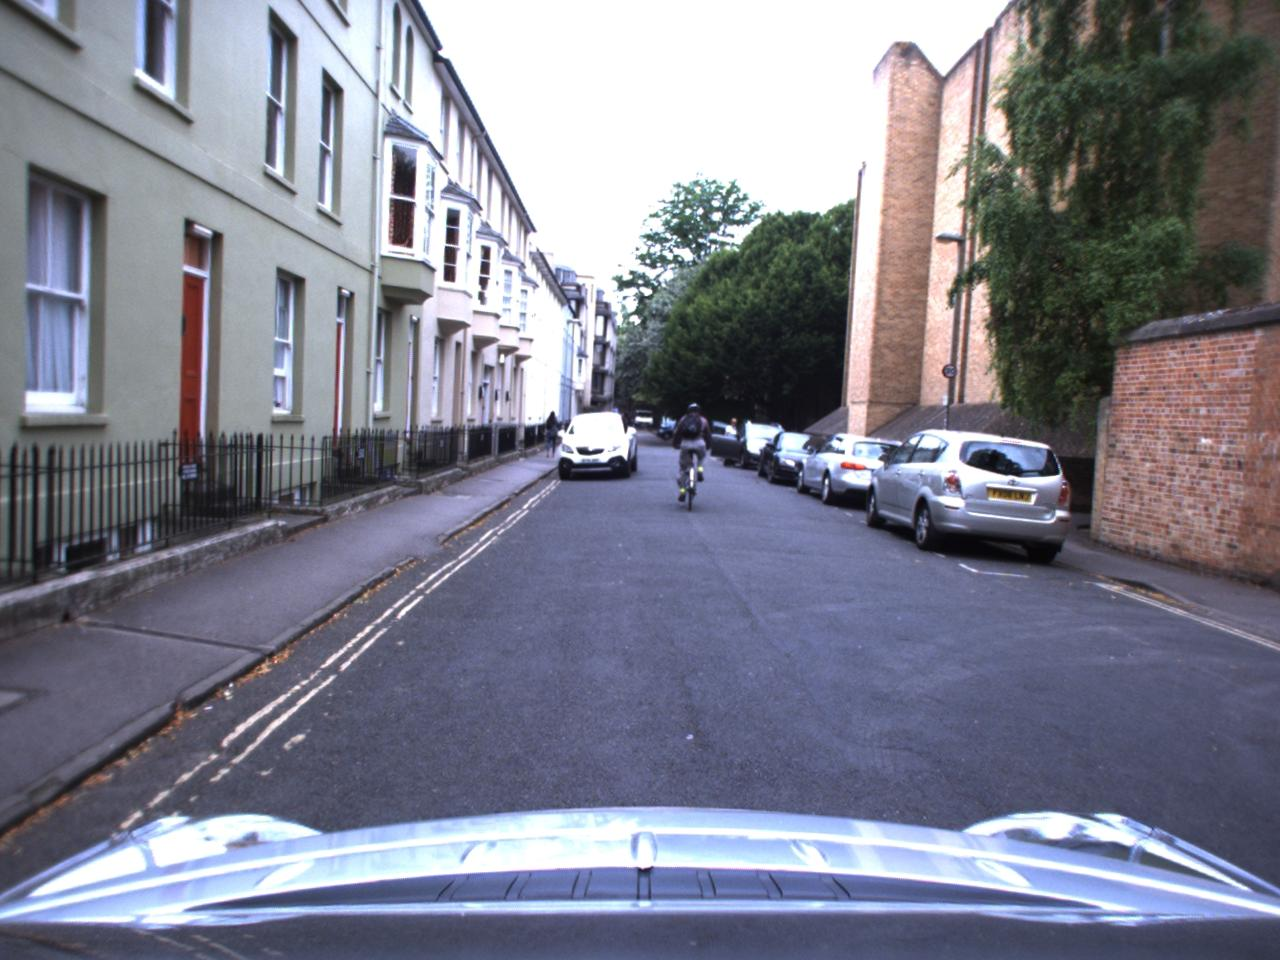
\includegraphics[width=0.12\linewidth]{ims_res/snow/q4/MAC.jpg}}
%\end{frame}

\begin{frame}{Results: long-term localization}
	\begin{minipage}{0.27\linewidth}
			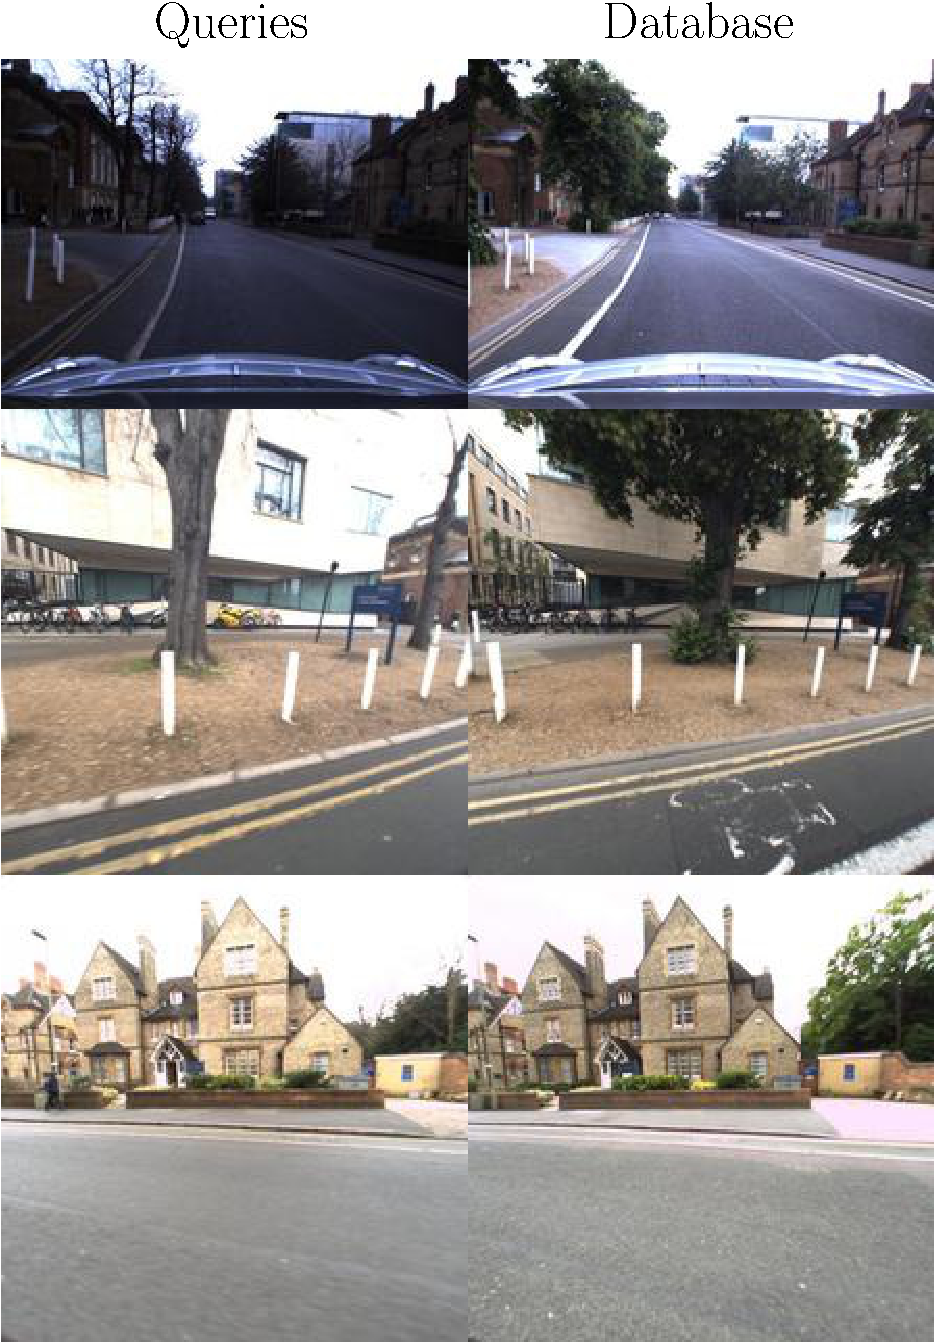
\includegraphics[width=\linewidth]{vect/res/dataset/lt_ex}
			\vfill

			{\scriptsize Example of queries and nearest image in the database.}
	\end{minipage}\hfill
	\begin{minipage}{0.49\linewidth}
		\centering
		\begin{figure}
			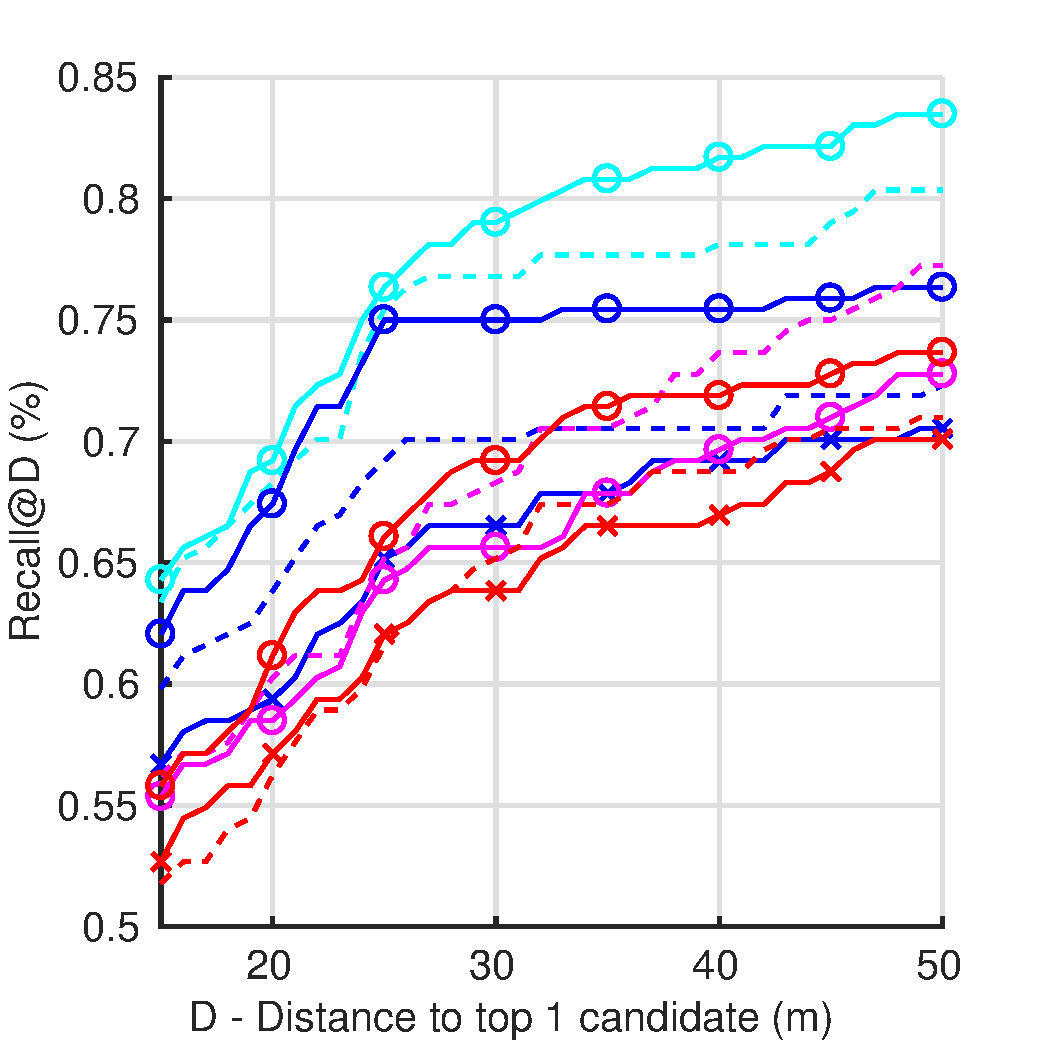
\includegraphics[width=0.9\linewidth]{vect/res/lt}
		\end{figure}
	\end{minipage}\hfill
	\begin{minipage}{0.2\linewidth}
			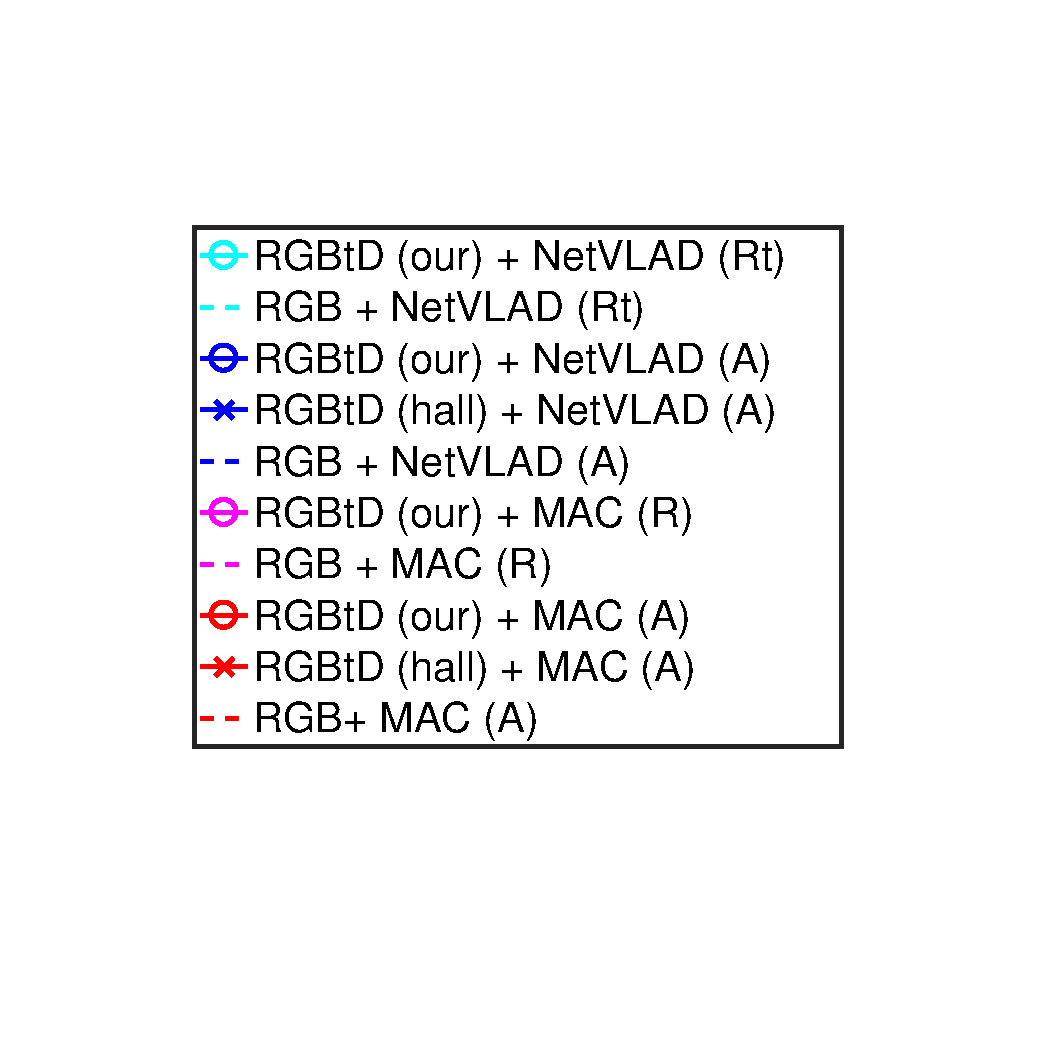
\includegraphics[trim={90 140 95 100},clip,width=\linewidth]{vect/res/legend}	
			\vspace{0.5cm}	
			{\scriptsize
			Competitors:
			\begin{itemize}
				\item[\textbf{-{}-{}-}] Only RGB [RGB]
				\item[\textbf{-x-}] Hallucination network [RGBtD (Hall)]
				\item[\textbf{-o-}] Our proposal [RGBtD (our)]
			\end{itemize}
			}
	\end{minipage}
\end{frame}

\begin{frame}{Results: cross-season localization}
	\begin{minipage}{0.27\linewidth}
			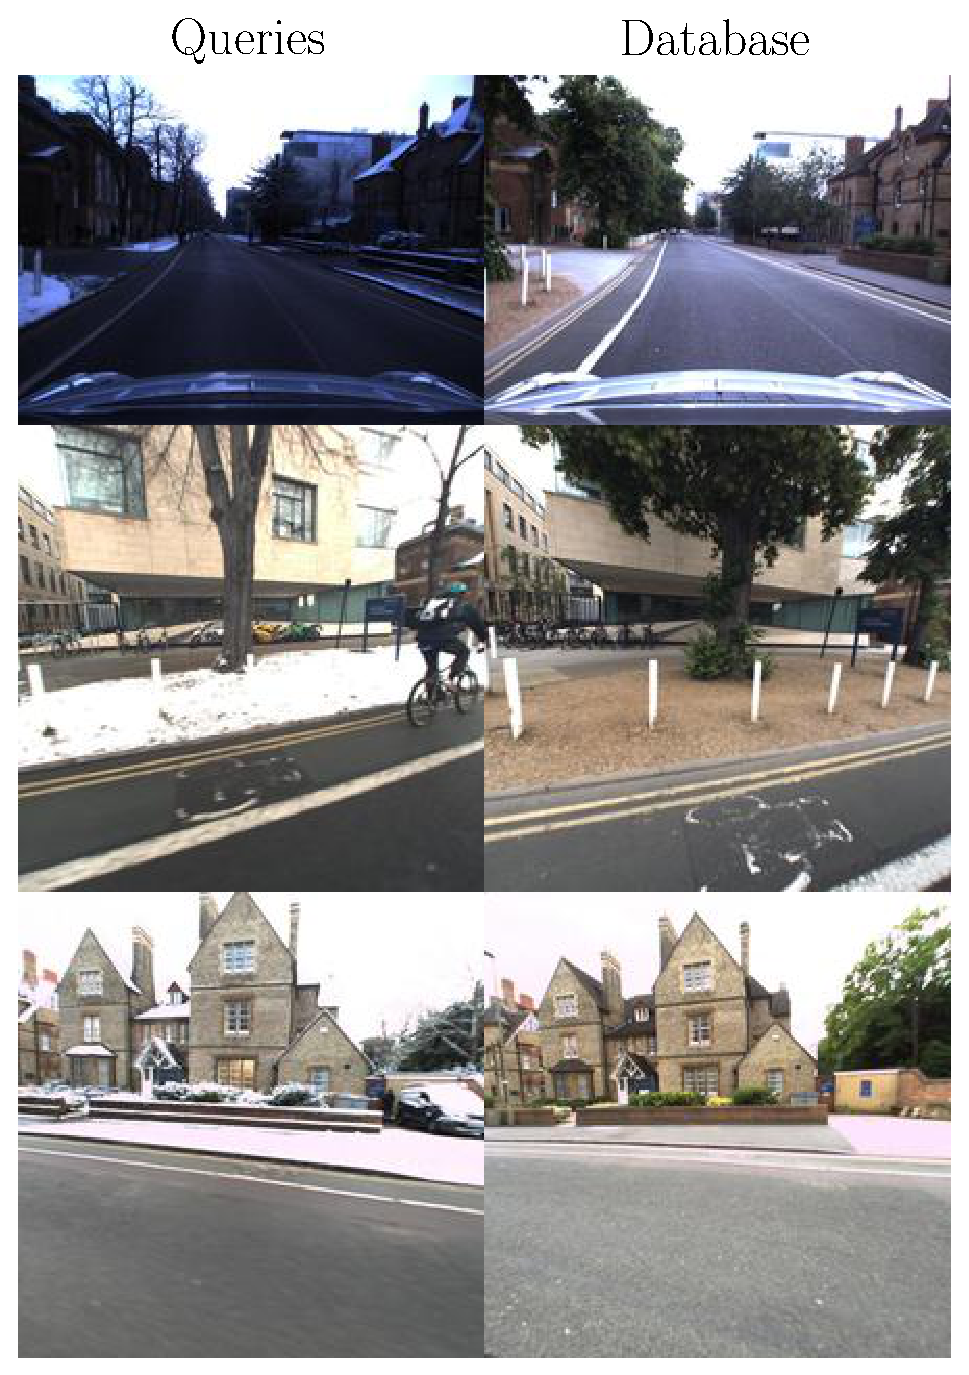
\includegraphics[width=\linewidth]{vect/res/dataset/snow_ex}
			\vfill

			{\scriptsize Example of queries and nearest image in the database.}
	\end{minipage}\hfill
	\begin{minipage}{0.49\linewidth}
		\centering
		\begin{figure}
			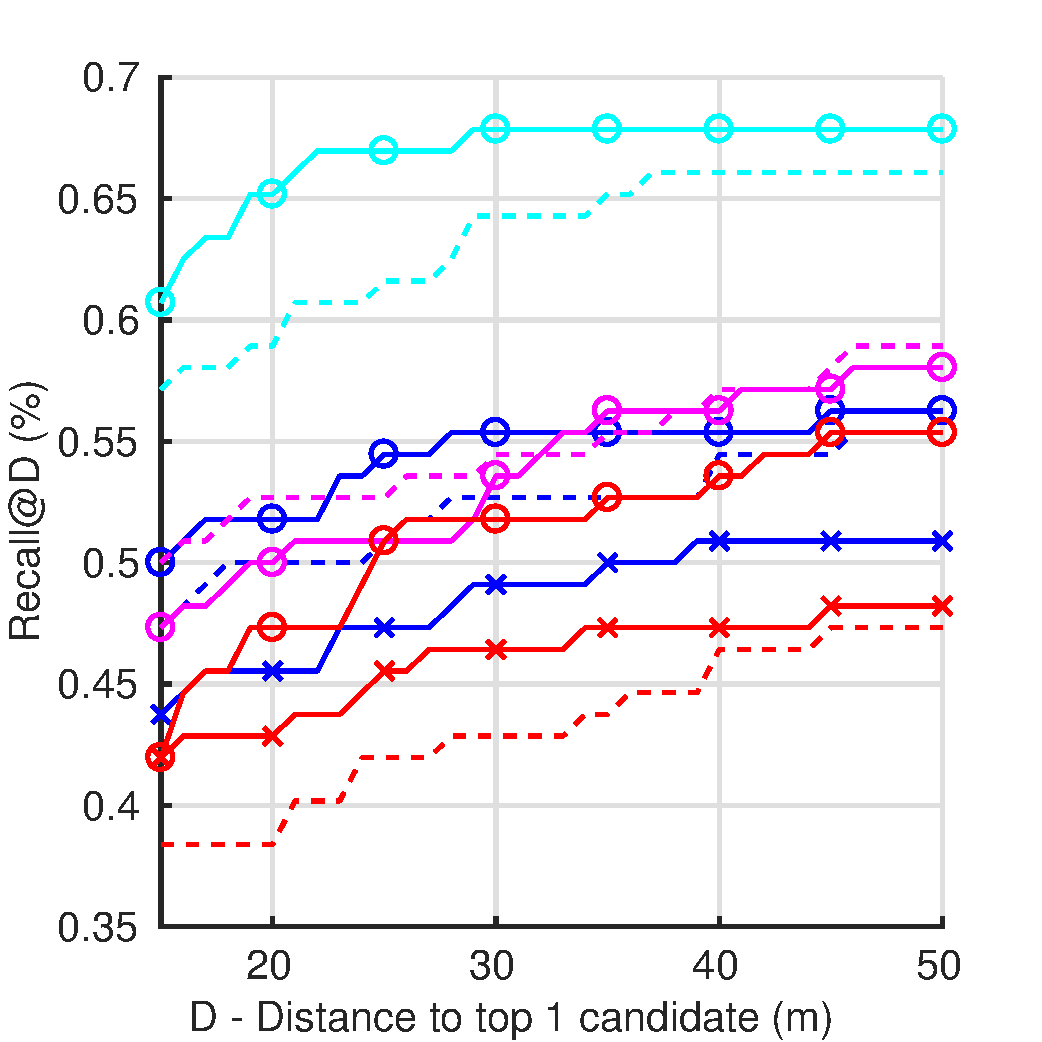
\includegraphics[width=0.9\linewidth]{vect/res/snow}
		\end{figure}
	\end{minipage}\hfill
	\begin{minipage}{0.2\linewidth}
			\includegraphics[trim={90 140 95 100},clip,width=\linewidth]{vect/res/legend}	
			\vspace{0.5cm}	
			{\scriptsize
			Competitors:
			\begin{itemize}
				\item[\textbf{-{}-{}-}] Only RGB [RGB]
				\item[\textbf{-x-}] Hallucination network [RGBtD (Hall)]
				\item[\textbf{-o-}] Our proposal [RGBtD (our)]
			\end{itemize}
			}
	\end{minipage}
\end{frame}

\begin{frame}{Failure case: Night to day}
	\begin{minipage}{0.27\linewidth}
			\includegraphics[width=\linewidth]{vect/res/dataset/night_ex}
			\vfill

			{\scriptsize Example of queries and nearest image in the database.}
	\end{minipage}\hfill
	\begin{minipage}{0.49\linewidth}
		\centering
		\begin{figure}
			\includegraphics[width=0.9\linewidth]{vect/res/night}
		\end{figure}
	\end{minipage}\hfill
	\begin{minipage}{0.2\linewidth}
			\includegraphics[trim={90 140 95 100},clip,width=\linewidth]{vect/res/legend}	
			\vspace{0.5cm}	
			{\scriptsize
			Competitors:
			\begin{itemize}
				\item[\textbf{-{}-{}-}] Only RGB [RGB]
				\item[\textbf{-x-}] Hallucination network [RGBtD (Hall)]
				\item[\textbf{-o-}] Our proposal [RGBtD (our)]
			\end{itemize}
			}
	\end{minipage}
\end{frame}


\begin{frame}{Improving night to day localization}
	\begin{minipage}{0.80\linewidth}
	\begin{figure}
		\centering
		\begin{minipage}{0.74\linewidth}
			\includegraphics[width=\linewidth]{im/res/night_input}
		\end{minipage}
		\begin{minipage}{0.25\linewidth}
			\raggedright \footnotesize
			{Night images that serve as input for the generative network}
		\end{minipage}
	\end{figure}
	\vspace{-0.5cm}
	\begin{figure}
		\centering
		\begin{minipage}{0.74\linewidth}
			\includegraphics[width=\linewidth]{im/res/night_gt}
		\end{minipage}
		\begin{minipage}{0.25\linewidth}
			\raggedright \footnotesize
			{Ground truth depth maps}
		\end{minipage}
	\end{figure}	
	\vspace{-0.5cm}
	\begin{figure}
		\centering
		\begin{minipage}{0.74\linewidth}
			\includegraphics[width=\linewidth]{im/res/night_noft}
		\end{minipage}
		\begin{minipage}{0.25\linewidth}
			\raggedright \footnotesize
			{Generated depth maps}
		\end{minipage}
	\end{figure}
	\end{minipage}
	\vfill

	\textbf{Our network is \textit{not able} to generate proper depth maps from night images.}
\end{frame}

\begin{frame}{Recall - Training policy}
	\begin{minipage}{0.6\linewidth}
		\centering
		\includegraphics[width=\linewidth]{vect/method/fig3/6d}	
	\end{minipage}\hfill
	\begin{minipage}{0.3\linewidth}
		\raggedright
		Thanks to the design of our method, we can improve generation performances of the decoder without impacting the descriptors networks.
		
		\uncover<2>{
		We fine tune our system with pairs of night image/depth map.
		\vspace{0.5cm}
		
		\includegraphics[width=\linewidth]{vect/res/fig1/night_pair}
		}
	\end{minipage}			
\end{frame}

\begin{frame}{Improving night to day localization}
\centering
\begin{minipage}{0.7\linewidth}
	\centering
	
	\begin{figure}
		\centering
		\begin{minipage}{0.74\linewidth}
			\includegraphics[width=\linewidth]{im/res/night_input}
		\end{minipage}
		\begin{minipage}{0.21\linewidth}
			\raggedright \footnotesize
			Night images that serve as input for the generative network
		\end{minipage}
	\end{figure}
	\vspace{-0.5cm}
	\begin{figure}
		\centering
		\begin{minipage}{0.74\linewidth}
			\includegraphics[width=\linewidth]{im/res/night_gt}
		\end{minipage}
		\begin{minipage}{0.21\linewidth}
			\raggedright \footnotesize
			Ground truth depth maps
		\end{minipage}
	\end{figure}	
	\vspace{-0.5cm}
	\begin{figure}
		\centering
		\begin{minipage}{0.74\linewidth}
			\includegraphics[width=\linewidth]{im/res/night_noft}
		\end{minipage}
		\begin{minipage}{0.21\linewidth}
			\raggedright \footnotesize
			Generated depth maps
		\end{minipage}
	\end{figure}
		\vspace{-0.5cm}
		\begin{figure}
			\centering
			\begin{minipage}{0.74\linewidth}
				\includegraphics[width=\linewidth]{im/res/night_ft}
			\end{minipage}
			\begin{minipage}{0.21\linewidth}
				\raggedright \footnotesize
				Generated depth maps, with fine tuning
			\end{minipage}
		\end{figure}
\end{minipage}
\end{frame}

\begin{frame}{Results: Night to day (fine tuning)}
	\begin{minipage}{0.49\linewidth}
		\centering
		\begin{figure}
			\includegraphics[width=0.9\linewidth]{vect/res/night}
			
			{Night vs daytime (w/o fine tuning)}
		\end{figure}
	\end{minipage}\hfill
	\begin{minipage}{0.49\linewidth}
		\centering
		\begin{figure}
			\includegraphics[width=0.9\linewidth]{vect/res/nightft}
			
			{Night vs daytime (w/ fine tuning)}
		\end{figure}
	\end{minipage}
	\vfill 
	
	{\small With fine tuning with a small amount of data, we are able to nearly double localization performances.}
\end{frame}
\section{Conclusion}

\label{sec:conclusion}

\begin{frame}{Conclusion}
	A new method for learning an image descriptor from side modality have been presented. Our descriptor performs especially well for challenging \textbf{cross-season} localization scenario, therefore it can be used to solve long-term place recognition problem. We additionally obtain encouraging results for \textbf{night to day} image retrieval.
	\vfill
	\uncover<2->
	{
	For future works:
	\begin{itemize}
		\item use other modalities,
		\item investigate less trivial descriptor fusion method,
		\item test on other visual localisation tasks (e.g. direct pose regression).
	\end{itemize}
	}
	\uncover<3->
	{
	\vfill	
	More details can be found in the associated paper\footfullcite{Piasco2019}.
	}	
\end{frame}

%\input{sections/posenet}
%\input{sections/dsac}
%\input{sections/dicp}

%%%%%%%%%%%%%%%%%%%%%%%%%%%%%%%%%%%%%%%%%%%%%%%%%%%%%%%%%%%%%%%%%%%%%%%%%%%%%%%%%%%%%%%
% Biblio
\begin{frame}[allowframebreaks,plain]
\frametitle{References}
\bibliographystyle{alpha_c}
\scriptsize{\bibliography{bib/mendeley.bib}}

\end{frame}

\appendix

\end{document}
